\chapter{Evaluation} \label{chapter:evaluation}
The verification of proposed solutions for machinery fault diagnostics is focused on two complementary activities, these are vibration measurement and defect identification. The accuracy of supervised learning using the k-nearest neighbour classifier is determined by the MaFaulDa dataset under various experiments. Data logger recording is compared to the known reference, and the collected Pump dataset is analyzed.

\section{MaFaulDa in k-nearest neighbors}
The four outlined experiments involve testing sets of features with very few members to see the effects in predictions when reducing the information content about machine status to the minimum. First, the attributes are left in the complete count after extraction. Then, all of their combinations are enumerated, and the resulting accuracy distribution is matched against accuracy after feature selection with similarity metrics. 

\subsection{Complete feature sets}
The two full sets of features include ten extracted from time-domain and eleven from frequency-domain of the vibrations. The feature spaces can incorrectly interchange different fault labels and better separate out some groups than the others. 

\begin{figure}[h]
    \centering
    \begin{subfigure}[b]{0.49\textwidth}
        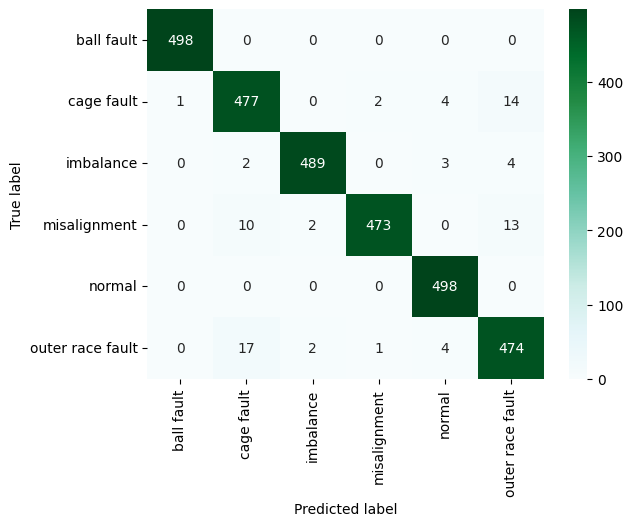
\includegraphics[width=\textwidth]{assets/results/all-features/TD-confusion-matrix.png}
        \caption{Time-domain features}
    \end{subfigure}
    \hfill
    \begin{subfigure}[b]{0.49\textwidth}
        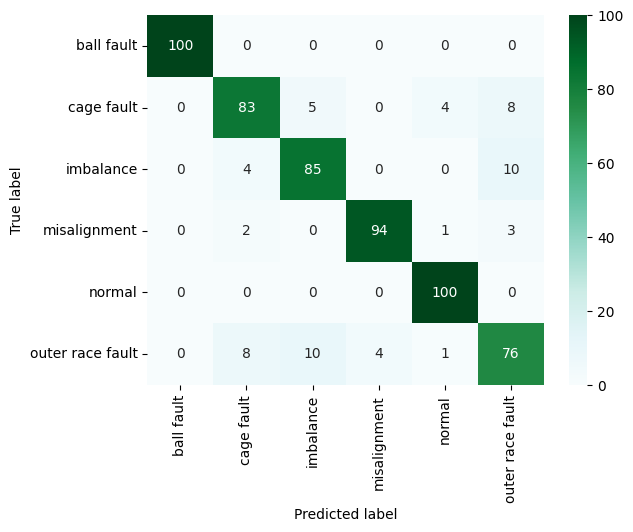
\includegraphics[width=\textwidth]{assets/results/all-features/FD-confusion-matrix.png}
        \caption{Frequency-domain features}
    \end{subfigure}
    \caption{Confusion matrix for complete sets of features}
    \label{fig:evaluation:all-features-confusion-matrix}
\end{figure}

The inner bearing observations are selected to train the k-NN with five neighbours and Euclidean distance metric. The attributes are normalized beforehand, rows are oversampled to a majority label, and data is split into training and testing sets with an 80:20 proportion. The 598 observation of validation data determines the confusion matrix (Fig.~\ref{fig:evaluation:all-features-confusion-matrix}). 

The label ``normal'' is not falsely attributed to other classes in either feature set, but other classes can get assigned to be ``normal''. Most mistakes happen while predicting outer race fault, which is confused with cage fault, imbalance, and less frequency with misalignment. The shaft imbalance is used for simulating bearing faults, which is a natural reason for this high error rate.

\begin{figure}[h]
    \centering
    \begin{subfigure}[b]{0.48\textwidth}
        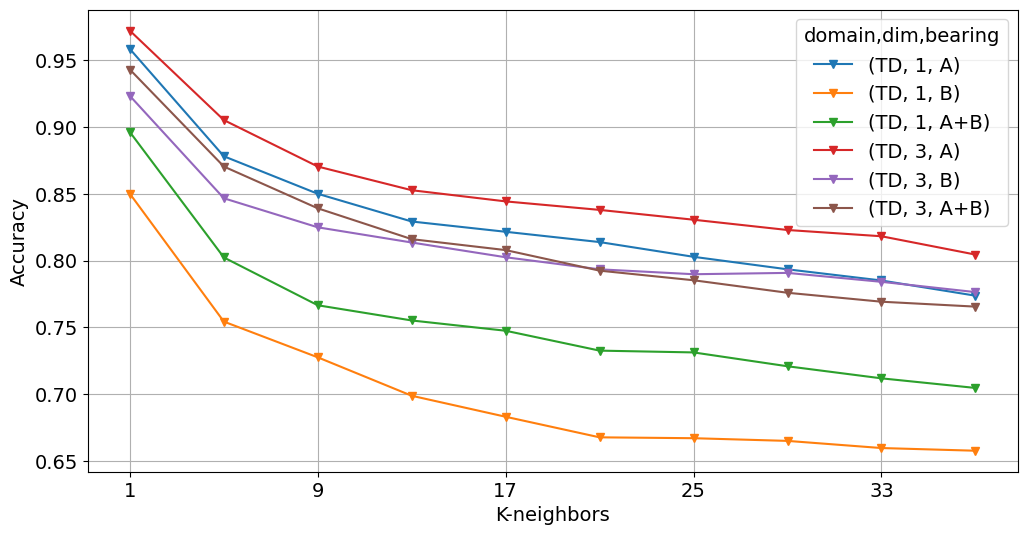
\includegraphics[width=\textwidth]{assets/results/all-features/TD.png}
        \caption{Time-domain features}
    \end{subfigure}
    \hfill
    \begin{subfigure}[b]{0.48\textwidth}
        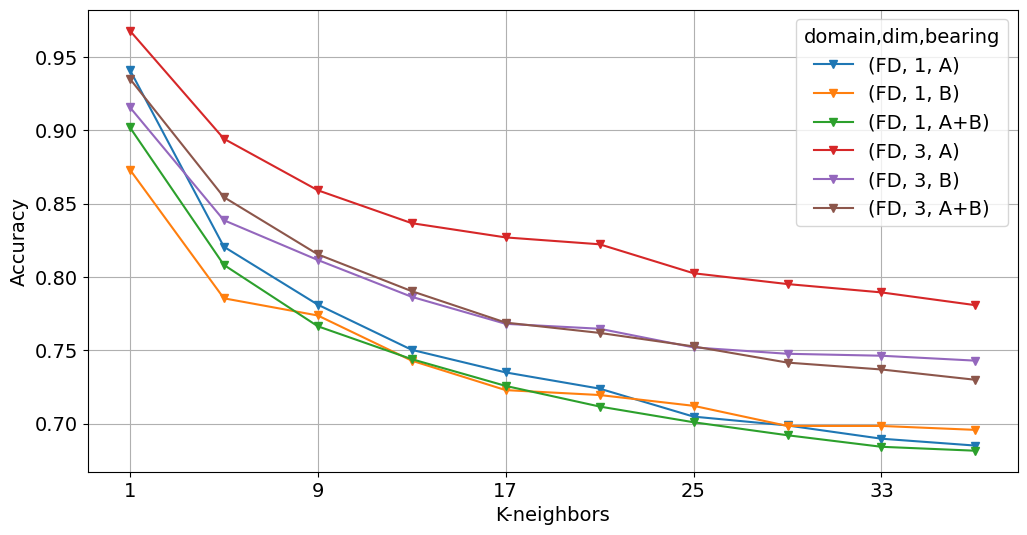
\includegraphics[width=\textwidth]{assets/results/all-features/FD.png}
        \caption{Frequency-domain features}
    \end{subfigure}
    \hfill
    \begin{subfigure}[b]{0.48\textwidth}
        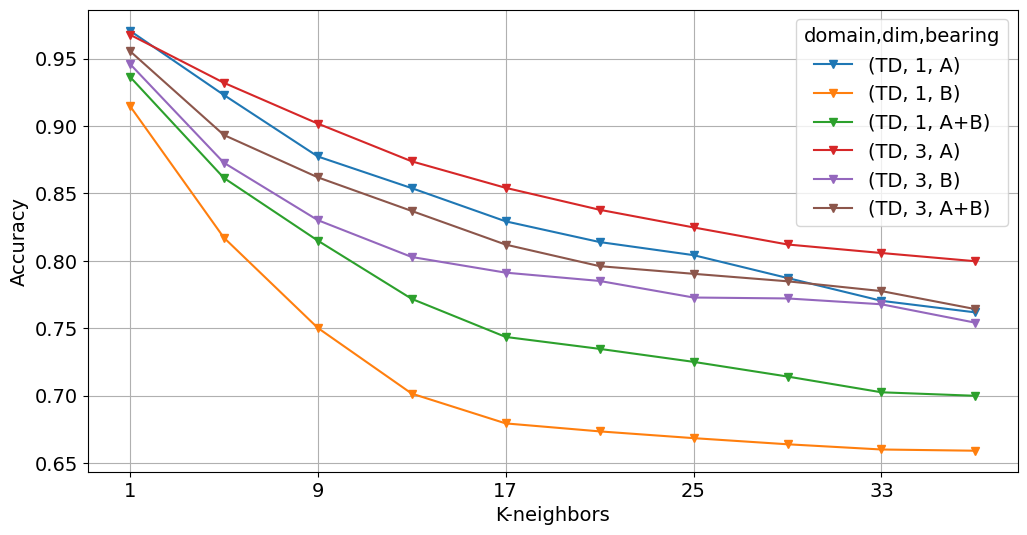
\includegraphics[width=\textwidth]{assets/results/all-features/TD-severity.png}
        \caption{Time-domain features (severity)}
    \end{subfigure}
    \hfill
    \begin{subfigure}[b]{0.48\textwidth}
        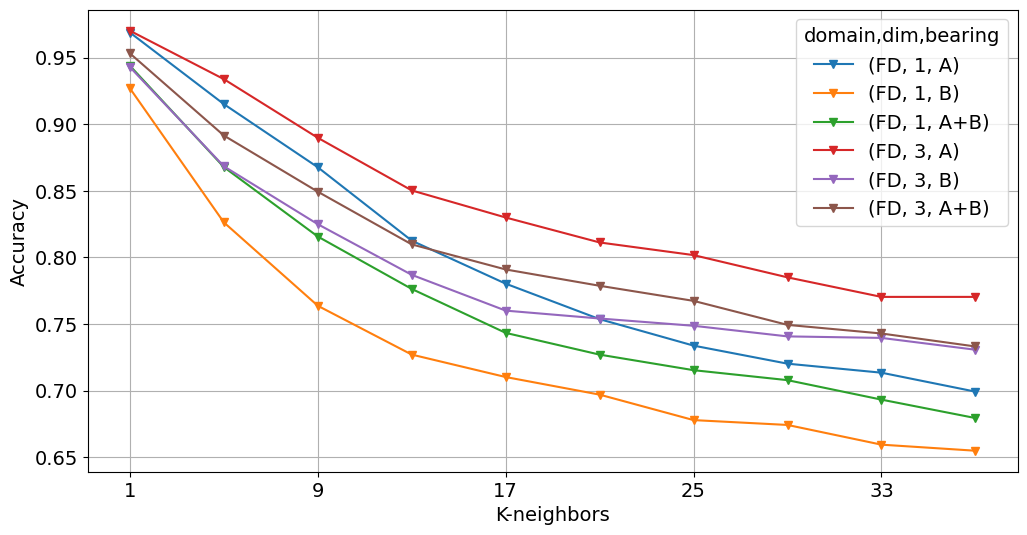
\includegraphics[width=\textwidth]{assets/results/all-features/FD-severity.png}
        \caption{Frequency-domain features (severity)}
    \end{subfigure} 
    \caption{Accuracy on complete feature sets depending on the k-value}
    \label{fig:evaluation:complete-set-k-value}
\end{figure}

The increasing number of neighbours used for classification in 5-fold cross-validated k-NN shows a substantial decrease in accuracy on validation sets (Fig.~\ref{fig:evaluation:complete-set-k-value}). The most prominent drop in performance of around 10\% occurs at the beginning until the k-value of nine, and then the accuracy curves slowly plateau.

Under every circumstance, the magnitude of the triaxial feature vector reaches better accuracy than those from only the axis of motion for the same source domain and bearing. The model for inner bearing A is more accurate than outer bearing B. The TD set is generally better in predictions than the FD set for the equivalent k-value. The relabeled dataset for high severity has a steeper decrease in accuracy for the same value of neighbours.


\subsection{Feature subset combinations}
The complete sets of predictors are even greatly shrunken to representation that could be presented in 3D plot or in perpendicular cross sections. These trend variables could be used in distingushing faults the same way as rms amplitude indicates their presence. Each possible combinations of pairs, triplets, and quadruplets constructs a separate k-NN model on which prediction accuracy is evaluated. 

\begin{figure}[h]
    \centering
    \begin{subfigure}[b]{0.48\textwidth}
        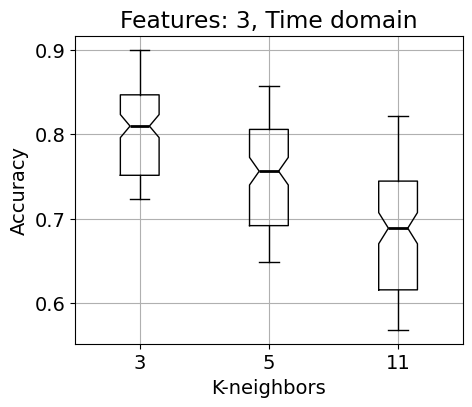
\includegraphics[width=\textwidth]{assets/results/feature-combinations/TD-3-A-False-False-F3.png}
        \caption{Three time-domain features}
    \end{subfigure}
    \hfill
    \begin{subfigure}[b]{0.48\textwidth}
        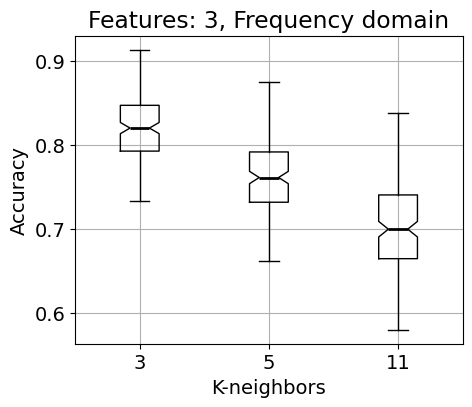
\includegraphics[width=\textwidth]{assets/results/feature-combinations/FD-3-A-False-False-F3.png}
        \caption{Three frequency-domain features}
    \end{subfigure}
    \hfill
    \begin{subfigure}[b]{0.48\textwidth}
        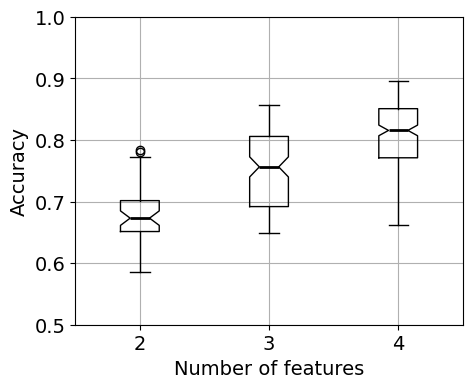
\includegraphics[width=\textwidth]{assets/results/feature-combinations/TD-3-A-False-False-K5.png}
        \caption{Five neighbours in time domain}
    \end{subfigure}
    \hfill
    \begin{subfigure}[b]{0.48\textwidth}
        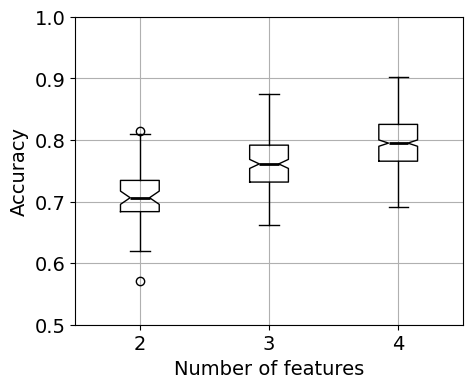
\includegraphics[width=\textwidth]{assets/results/feature-combinations/FD-3-A-False-False-K5.png}
        \caption{Five neighbours in frequency domain}
    \end{subfigure}
    \caption{Model accuracy distribution for bearing A and three axis features}
    \label{fig:evaluation:model-accuracy}
\end{figure}

\begin{figure}[h]
    \centering
    \begin{subfigure}[b]{0.48\textwidth}
        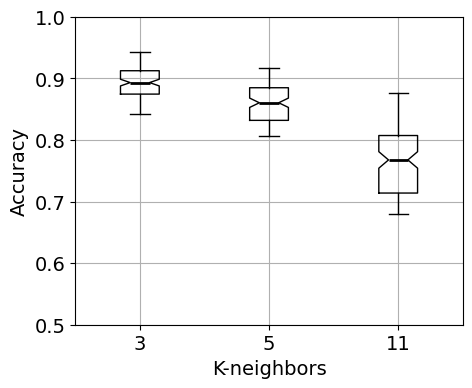
\includegraphics[width=\textwidth]{assets/results/feature-combinations/TD-3-A-True-False-F3.png}
        \caption{Three time-domain features}
    \end{subfigure}
    \hfill
    \begin{subfigure}[b]{0.48\textwidth}
        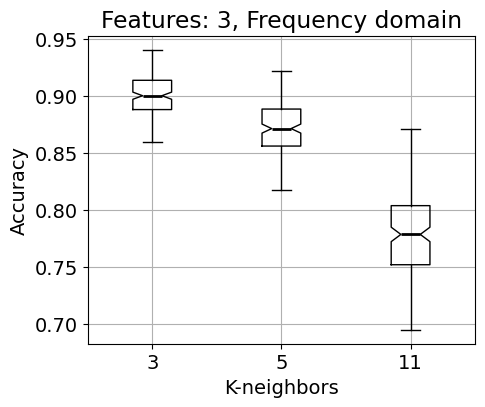
\includegraphics[width=\textwidth]{assets/results/feature-combinations/FD-3-A-True-False-F3.png}
        \caption{Three frequency-domain features}
    \end{subfigure}
    \hfill
    \begin{subfigure}[b]{0.48\textwidth}
        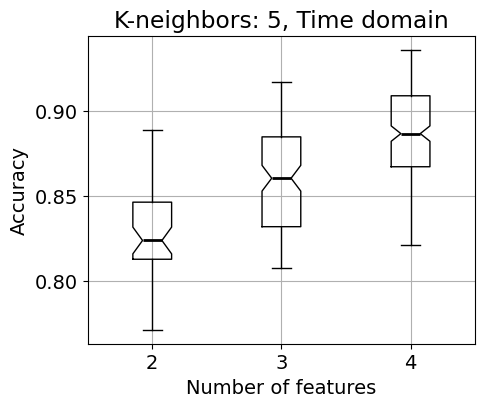
\includegraphics[width=\textwidth]{assets/results/feature-combinations/TD-3-A-True-False-K5.png}
        \caption{Five neighbours in time domain}
    \end{subfigure}
    \hfill
    \begin{subfigure}[b]{0.48\textwidth}
        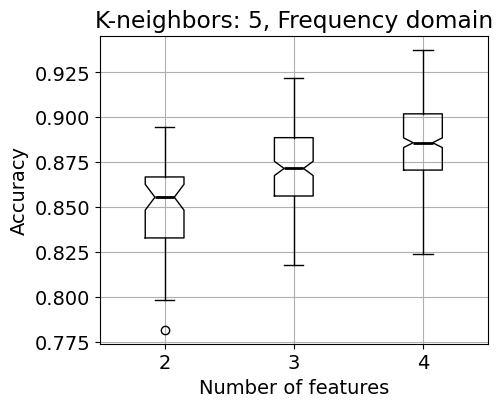
\includegraphics[width=\textwidth]{assets/results/feature-combinations/FD-3-A-True-False-K5.png}
        \caption{Five neighbours in frequency domain}
    \end{subfigure}
    \caption{Model accuracy distribution from bearing A and three axis features after relabeling for high severity faults}
    \label{fig:evaluation:model-accuracy-severity}
\end{figure}

The distribution of model accuracies is documented on features in both domains coined from three dimensions on bearing A with original and high-severity defect labels. The boxplots display the relation of the k-value to accuracy when three features are chosen, and the relation of a number of features to accuracy with five neighbours(Fig.~\ref{fig:evaluation:model-accuracy-severity} and \ref{fig:evaluation:model-accuracy-severity}).

The decrease in accuracy with additional neighbours is apparent and similar to the trend in complete sets of features. We are interested in maximum accuracy in the distribution because that is the optimal model feature selection method to try to approach. Its reduction is more noticeable between three and five features 3 - 5\%, and almost the same amount between five and eleven neighbours. 

The complete sets reach better accuracy than subsets when the number of features is at most three and simultaneously the number of neighbours is five or less. For more triaxial features and more neighbours, the complete set is only about 2\% percent worse at the most than subsets because the curse of dimensionality is not so substantial for ten dimensions.

The spread in model accuracies in the interquartile range is from 5 to 10 \%, and measured between whiskers is at a maximum of 25\%. The standard deviation is about 7\%. Overall, the time-domain features are better than frequency-domain features for these specific feature spaces.

The number of features has a direct proportionality effect on the optimal model accuracy. An increase from two to three features has more weight than allowing a fourth attribute. The contributions of adding features are around 6\% and 3\%, and the relabeled dataset has an increase of 3\% and 2\%. The absolute accuracies are consecutively for 2, 3, and 4 features when k is equal to 5: 78.31\%, 85.67\%, and 89.55\% for the time domain and 81.52\%, 87.52\%, 90.26\% in the frequency domain.


\subsection{Feature selection techniques}
The predictors chosen with supervised selection strategies are compared in accuracy and location within the accuracy distribution of exhaustive combinations of same-sized sets and the performance of its source superset. The metrics for bivariate feature selection are correlation, F statistic, mutual information, and their ensemble by the rank product. The PCA of the complete feature set that retains the same number of features and selection methods serves as a benchmark to tell whether the linear combination or subset gets better performance on the MaFaulDa.

\begin{table}[h]
\centering
\begin{adjustbox}{width=\textwidth}
\begin{tabular}{|l|rr|rr|r|l|}
\hline
\multirow{2}{*}{\textbf{Feature set}} & \multicolumn{2}{l|}{\textbf{Accuracy}}                                   & \multicolumn{2}{l|}{\textbf{Percentile}}                 & \multicolumn{1}{l|}{\multirow{2}{*}{\textbf{Domain}}} & \multirow{2}{*}{\textbf{Best features}} \\ \cline{2-5}
                                      & \multicolumn{1}{l|}{\textbf{Train}} & \multicolumn{1}{l|}{\textbf{Test}} & \multicolumn{1}{l|}{\textbf{Train}} & \multicolumn{1}{l|}{\textbf{Test}} & \multicolumn{1}{l|}{}                               &                                         \\ \hline
All features                          & \multicolumn{1}{r|}{96.03}          & 92.80                              & \multicolumn{1}{r|}{100.00}         & 100.00                             & TD                                                   &                                         \\ \hline
PCA PC                                & \multicolumn{1}{r|}{91.20}          & 84.67                              & \multicolumn{1}{r|}{95.00}          & 93.33                              & TD                                                   &                                         \\ \hline
Best features                         & \multicolumn{1}{r|}{91.93}          & 85.47                              & \multicolumn{1}{r|}{100.00}         & 99.17                              & TD                                                   & zerocross, pp, skewness                 \\ \hline
Rank product                          & \multicolumn{1}{r|}{91.21}          & 85.04                              & \multicolumn{1}{r|}{95.83}          & 97.50                              & TD                                                   & zerocross, shape, rms                   \\ \hline
Correlation                           & \multicolumn{1}{r|}{91.21}          & 85.04                              & \multicolumn{1}{r|}{95.83}          & 97.50                              & TD                                                   & shape, zerocross, rms                   \\ \hline
F statistic                           & \multicolumn{1}{r|}{90.59}          & 84.07                              & \multicolumn{1}{r|}{91.67}          & 90.00                              & TD                                                   & rms, pp, zerocross                      \\ \hline
Mutual information                    & \multicolumn{1}{r|}{88.24}          & 80.62                              & \multicolumn{1}{r|}{75.83}          & 76.67                              & TD                                                   & zerocross, shape, crest                 \\ \hline
All features                          & \multicolumn{1}{r|}{93.67}          & 88.45                              & \multicolumn{1}{r|}{100.00}         & 100.00                             & FD                                                  &                                         \\ \hline
PCA PC                                & \multicolumn{1}{r|}{86.76}          & 78.51                              & \multicolumn{1}{r|}{64.85}          & 70.91                              & FD                                                   &                                         \\ \hline
Best features                         & \multicolumn{1}{r|}{92.86}          & 87.52                              & \multicolumn{1}{r|}{100.00}         & 100.00                             & FD                                                   & centroid, roll\_off, entropy            \\ \hline
Rank product                          & \multicolumn{1}{r|}{85.79}          & 77.18                              & \multicolumn{1}{r|}{51.52}          & 57.58                              & FD                                                   & roll\_off, flux, skewness               \\ \hline
Correlation                           & \multicolumn{1}{r|}{85.79}          & 77.18                              & \multicolumn{1}{r|}{51.52}          & 57.58                              & FD                                                   & roll\_off, skewness, flux               \\ \hline
F statistic                           & \multicolumn{1}{r|}{85.79}          & 77.18                              & \multicolumn{1}{r|}{51.52}          & 57.58                              & FD                                                   & roll\_off, flux, skewness               \\ \hline
Mutual information                    & \multicolumn{1}{r|}{90.73}          & 83.60                              & \multicolumn{1}{r|}{94.55}          & 94.55                              & FD                                                   & roll\_off, entropy, noisiness           \\ \hline
\end{tabular}
\end{adjustbox}
\caption{Feature selection method accuracy and percentile within accuracy distribution of all three member subsets. (bearing = A, dimension = 3, k=5)}
\label{tab:evaluation:fsel}
\end{table}

\begin{table}[h]
\centering
\begin{adjustbox}{width=\textwidth}
\begin{tabular}{|l|rr|rr|r|l|}
\hline
\multirow{2}{*}{\textbf{Feature set}} & \multicolumn{2}{l|}{\textbf{Accuracy}}                                   & \multicolumn{2}{l|}{\textbf{Percentile}}                 & \multicolumn{1}{l|}{\multirow{2}{*}{\textbf{Domain}}} & \multirow{2}{*}{\textbf{Best features}} \\ \cline{2-5}
                                      & \multicolumn{1}{l|}{\textbf{Train}} & \multicolumn{1}{l|}{\textbf{Test}} & \multicolumn{1}{l|}{\textbf{Train}} & \multicolumn{1}{l|}{\textbf{Test}} & \multicolumn{1}{l|}{}                               &                                         \\ \hline
All features                          & \multicolumn{1}{r|}{96.42}          & 94.76                              & \multicolumn{1}{r|}{100.00}         & 100.00                             & TD                                                   &                                         \\ \hline
PCA PC                                & \multicolumn{1}{r|}{94.63}          & 92.07                              & \multicolumn{1}{r|}{100.00}         & 100.00                             & TD                                                   &                                         \\ \hline
Best features                         & \multicolumn{1}{r|}{94.58}          & 91.71                              & \multicolumn{1}{r|}{100.00}         & 99.17                              & TD                                                   & zerocross, aac, shape                   \\ \hline
Rank product                          & \multicolumn{1}{r|}{94.31}          & 91.40                              & \multicolumn{1}{r|}{98.33}          & 95.83                              & TD                                                   & zerocross, shape, rms                   \\ \hline
Correlation                           & \multicolumn{1}{r|}{94.31}          & 91.40                              & \multicolumn{1}{r|}{98.33}          & 95.83                              & TD                                                   & zerocross, shape, rms                   \\ \hline
F statistic                           & \multicolumn{1}{r|}{94.31}          & 91.40                              & \multicolumn{1}{r|}{98.33}          & 95.83                              & TD                                                   & shape, zerocross, rms                   \\ \hline
Mutual information                    & \multicolumn{1}{r|}{91.90}          & 88.51                              & \multicolumn{1}{r|}{72.50}          & 76.67                              & TD                                                   & zerocross, shape, clearance             \\ \hline
All features                          & \multicolumn{1}{r|}{95.20}          & 93.20                              & \multicolumn{1}{r|}{100.00}         & 100.00                             & FD                                                   &                                         \\ \hline
PCA PC                                & \multicolumn{1}{r|}{92.14}          & 88.84                              & \multicolumn{1}{r|}{69.09}          & 73.94                              & FD                                                   &                                         \\ \hline
Best features                         & \multicolumn{1}{r|}{94.64}          & 91.94                              & \multicolumn{1}{r|}{100.00}         & 99.39                              & FD                                                   & centroid, roll\_off, entropy            \\ \hline
Rank product                          & \multicolumn{1}{r|}{93.89}          & 91.24                              & \multicolumn{1}{r|}{95.15}          & 97.58                              & FD                                                   & entropy, noisiness, centroid            \\ \hline
Correlation                           & \multicolumn{1}{r|}{94.50}          & 92.19                              & \multicolumn{1}{r|}{99.39}          & 100.00                             & FD                                                   & entropy, centroid, flux                 \\ \hline
F statistic                           & \multicolumn{1}{r|}{94.50}          & 92.19                              & \multicolumn{1}{r|}{99.39}          & 100.00                             & FD                                                   & entropy, flux, centroid                 \\ \hline
Mutual information                    & \multicolumn{1}{r|}{93.32}          & 90.67                              & \multicolumn{1}{r|}{90.91}          & 91.52                              & FD                                                   & noisiness, roll\_off, entropy           \\ \hline
\end{tabular}
\end{adjustbox}
\caption{Feature selection method accuracy and percentile within accuracy distribution of all three member subsets. (severity, bearing = A, dimension = 3, k=5)}
\label{tab:evaluation:fsel-severity}
\end{table}

Table~\ref{tab:evaluation:fsel} compares the concrete case of choosing the three features from each domain on bearing A and k-NN with five neighbours. Table~\ref{tab:evaluation:fsel-severity} uses labels for high-severity faults. There is a significant difference in train and test accuracy, which means the model is likely overfitting. The percentile within the distribution is measured to its respective data, the train or validation set. However, the percentile of best features in the test is calculated against train distribution.

Combining the rankings from several metrics is necessary to get consistent results. This is evidenced by the variability of the success of selected feature sets in final prediction performance under multiple conditions. The PCA with 3 components out of complete feature sets is comparable in accuracy to selection methods with original attributes.

The triplet of variables with the best results is from TD set: zero-crossing rate, peak-to-peak, skewness, and from FD set: centroid, roll-off, and entropy. With high severity labels, the best attributes for FD stay the same, but average amplitude change and shape factor are preferred along the zero-crossing rate. The rank product picked up roll-off, flux, and skewness for the FD set, which is suboptimal. The two of the three methods in the ensemble arrive at the same set overruling the superior set produced by mutual information. In the TD set, the zero-crossing rate, shape, and rms, are chosen by rank product. 

\begin{figure}[h]
    \centering
    \begin{subfigure}[b]{0.48\textwidth}
        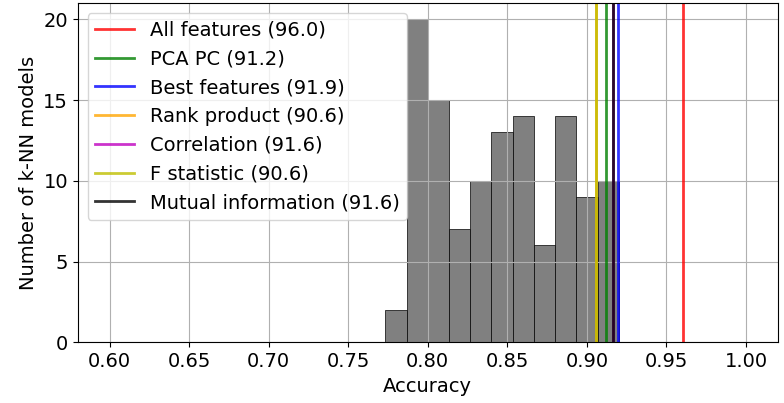
\includegraphics[width=\textwidth]{assets/results/feature-combinations/model-distr-fsel-k5-f3-TD-train.png}
        \caption{Time-domain features (train)}
    \end{subfigure}
    \hfill
    \begin{subfigure}[b]{0.48\textwidth}
        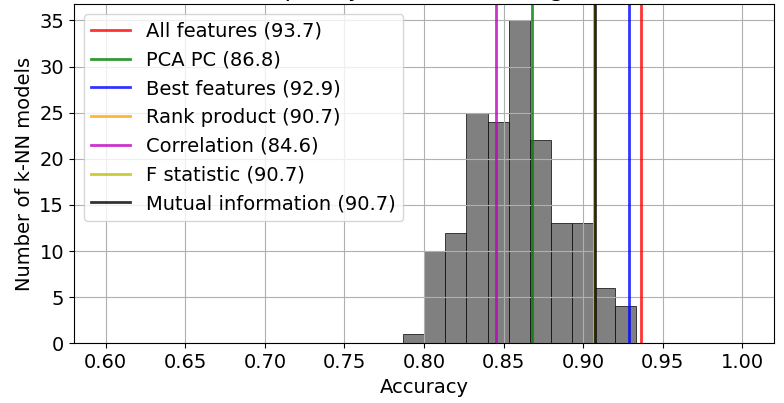
\includegraphics[width=\textwidth]{assets/results/feature-combinations/model-distr-fsel-k5-f3-FD-train.png}
        \caption{Frequency-domain features (train)}
    \end{subfigure}
    \hfill
    \begin{subfigure}[b]{0.48\textwidth}
        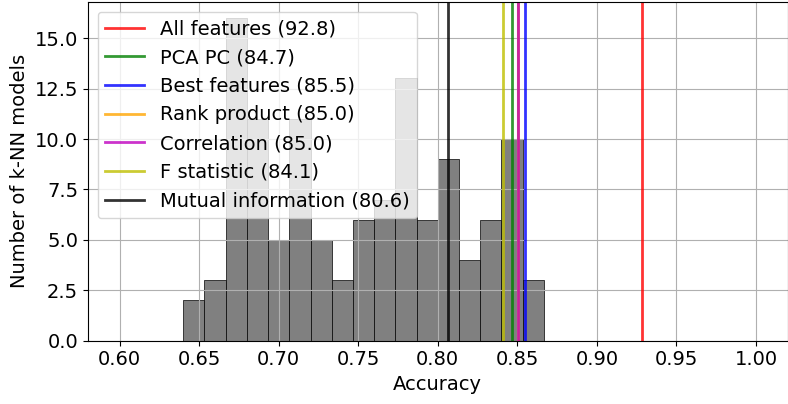
\includegraphics[width=\textwidth]{assets/results/feature-combinations/model-distr-fsel-k5-f3-TD-test.png}
        \caption{Time-domain features (test)}
    \end{subfigure}
    \hfill
    \begin{subfigure}[b]{0.48\textwidth}
        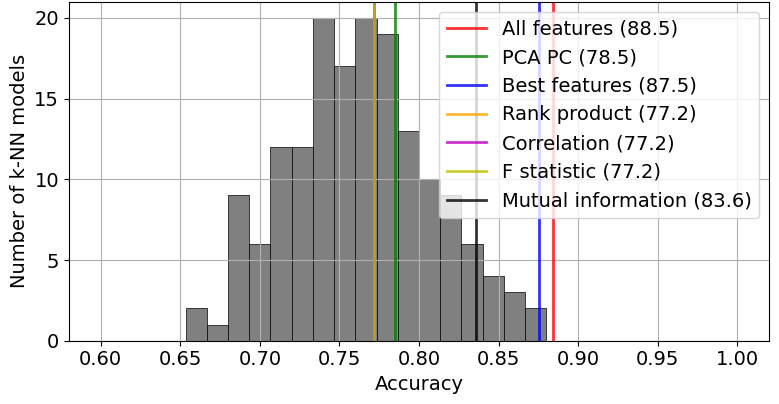
\includegraphics[width=\textwidth]{assets/results/feature-combinations/model-distr-fsel-k5-f3-FD-test.png}
        \caption{Frequency-domain features (test)}
    \end{subfigure}
    \caption{Model accuracy statistical distibutions with feature selection methods for three predictors (k = 5)}
    \label{fig:evaluation:fsel-model-distr}
\end{figure}

The entire accuracy distribution for the training and testing set for original labels is drawn in the form of the histogram (Fig.~\ref{fig:evaluation:fsel-model-distr}). The results of the chosen predictors are mapped out onto the distribution as vertical lines that stack up near the maximum for the time domain or disperse slightly above the median for the frequency domain. The accuracy of all features is unreachable for three feature subsets. Another noticeable difference between distributions is their shift down and greater spread in testing compared to training sets.

\begin{table}[h]
\centering
\begin{adjustbox}{width=\textwidth}
\begin{tabular}{|l|r|r|}
\hline
\textbf{Method}    & \multicolumn{1}{l|}{\textbf{Median percentile {[}\%{]}}} & \multicolumn{1}{l|}{\textbf{Median accuracy {[}\%{]}}} \\ \hline
Rank product       & 88.97                                                    & 79.82                                                 \\ \hline
Mutual information & 91.81                                                    & 80.87                                                 \\ \hline
F statistic        & 86.90                                                    & 79.63                                                 \\ \hline
Correlation        & 84.49                                                    & 79.04                                                  \\ \hline
\end{tabular}
\end{adjustbox}
\caption{Feature selection methods evaluated in summary over all experimental conditions}
\label{tab:evaluation:compare-fsel-accuracy}
\end{table}

\begin{table}[h]
\centering
\begin{adjustbox}{width=\textwidth}
\begin{tabular}{|l|r|r|r|}
\hline
                            & \multicolumn{1}{l|}{\textbf{Best in scenarios}} & \multicolumn{1}{l|}{\textbf{Scenarios {[}\%{]}}} & \multicolumn{1}{l|}{\textbf{Mean percentile {[}\%{]}}} \\ \hline
\textbf{Rank product}       & 94                                                     & 43.52                                            & 92.38 \\ \hline
\textbf{Mutual information} & 87                                                      & 40.28                                            & 91.79 \\ \hline
\textbf{Correlation}        & 26                                                      & 12.04                                             & 97.54 \\ \hline
\textbf{F statistic}        & 9                                                       & 4.16                                             & 96.10 \\ \hline
\textbf{$\Sigma$}           & 216                                                     & 100                                       & -                                                      \\ \hline
\end{tabular}
\end{adjustbox}
\caption{The experimental scenarios in which the method is found to be the best}
\label{tab:evaluation:best-selection-method}
\end{table}

\begin{figure}[h]
    \centering
    \begin{subfigure}[b]{0.48\textwidth}
        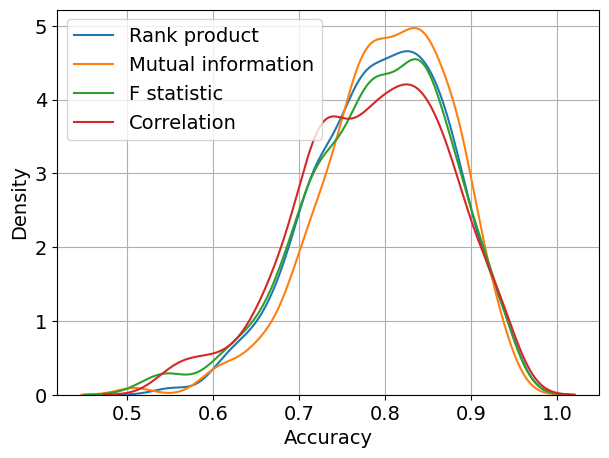
\includegraphics[width=\textwidth]{assets/results/feature-combinations/fsel-accuracy.png}
        \caption{Accuracy}
    \end{subfigure}
    \hfill
    \begin{subfigure}[b]{0.48\textwidth}
        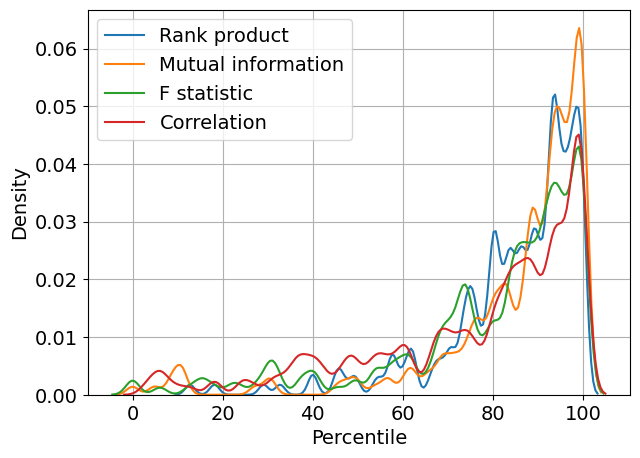
\includegraphics[width=\textwidth]{assets/results/feature-combinations/fsel-percentile.png}
        \caption{Percentile}
    \end{subfigure}
    \caption{Quality of choice for feature selection methods}
    \label{fig:evaluation:kde-fsel-perecentile}
\end{figure}

Under 216 scenarios, the mutual information has better median accuracy (80.87\%) and distribution percentile (91.81\%) followed by rank product with an accuracy of 79.82\% of and percentile of 88.97\% (Tab.~\ref{tab:evaluation:compare-fsel-accuracy}). The scenarios are composed of 24 base dataset modifications and options for hyperparameters k-value and number of features. 

The rank product was the best method in the majority of 43.52\% scenarios. Mutual information comes second in 40.28\% cases, where it is deemed the best strategy (Tab.~\ref{tab:evaluation:best-selection-method}). The median accuracy in selected cases is also better for rank product 92.38\% compared to 91.79\% mutual information. 

Kernel density estimate plot (Fig.~\ref{fig:evaluation:kde-fsel-perecentile}) shows the distribution of accuracies for the selection methods and percentiles for predictor subsets they chose. The feature selection usually picks variables so that they stay in the upper quartile of the distribution above the 75\% percentile. The median accuracy of all methods is around the vicinity of 80\%.

\begin{figure}[h]
    \centering
    \begin{subfigure}[b]{0.48\textwidth}
        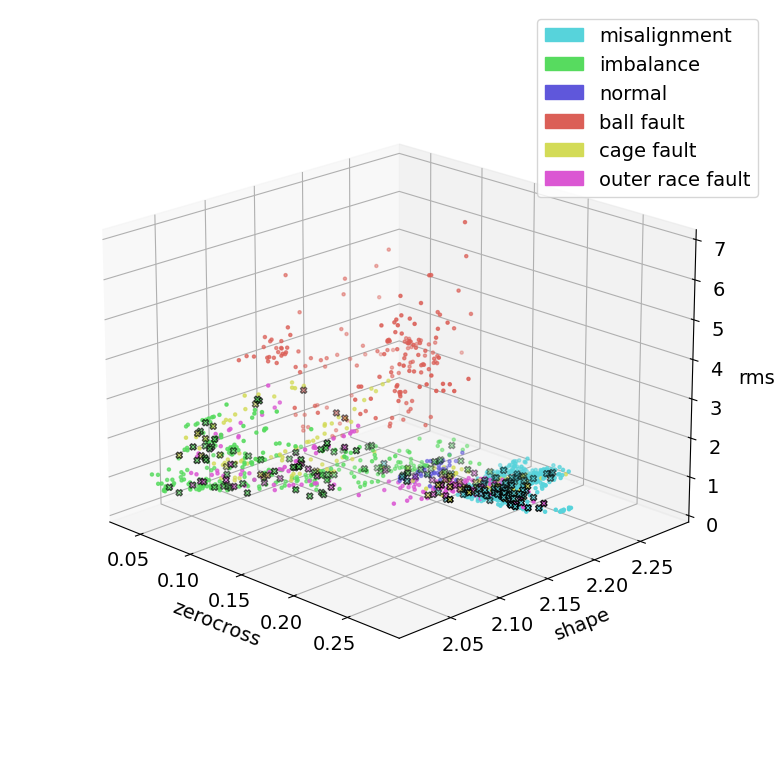
\includegraphics[width=\textwidth]{assets/results/labels/TD.png}
        \caption{Time-domain features [89.05\%]}
    \end{subfigure}
    \hfill
    \begin{subfigure}[b]{0.48\textwidth}
        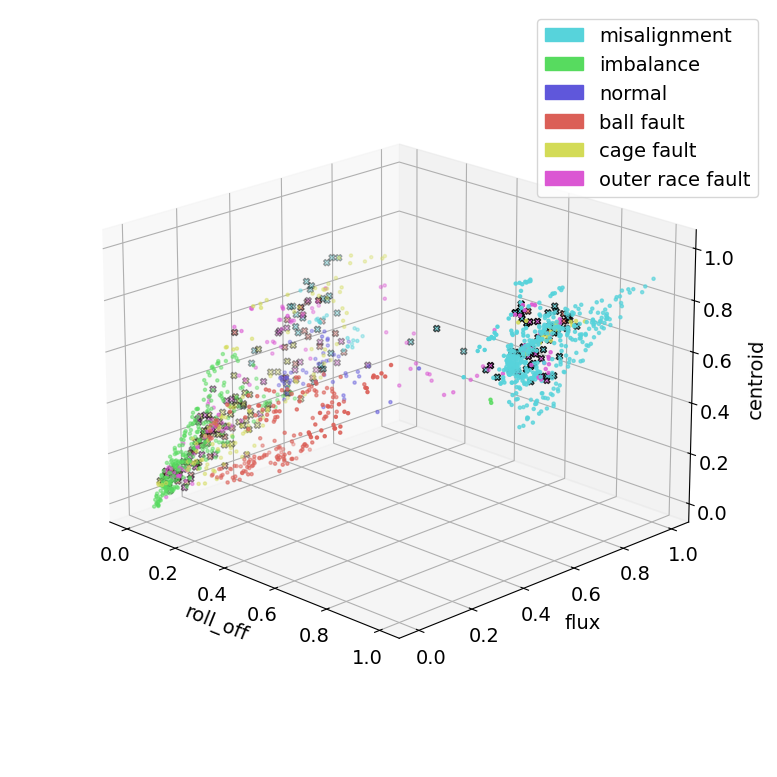
\includegraphics[width=\textwidth]{assets/results/labels/FD.png}
        \caption{Frequency-domain features [77.18\%]}
    \end{subfigure}
    \hfill
    \begin{subfigure}[b]{0.48\textwidth}
        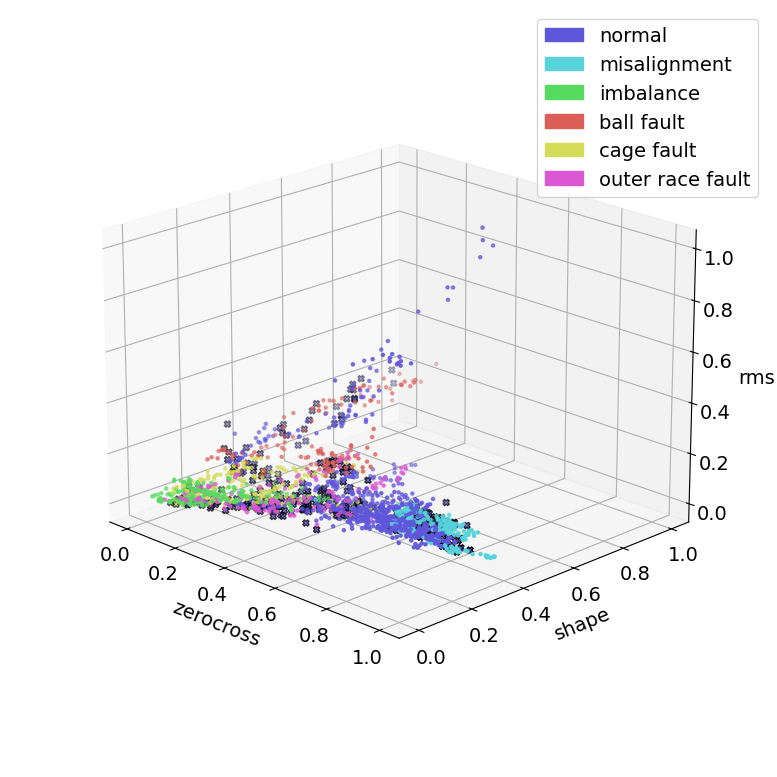
\includegraphics[width=\textwidth]{assets/results/labels/TD-severity.png}
        \caption{Time-domain features (severity) [91.40\%]}
    \end{subfigure}
    \hfill
    \begin{subfigure}[b]{0.48\textwidth}
        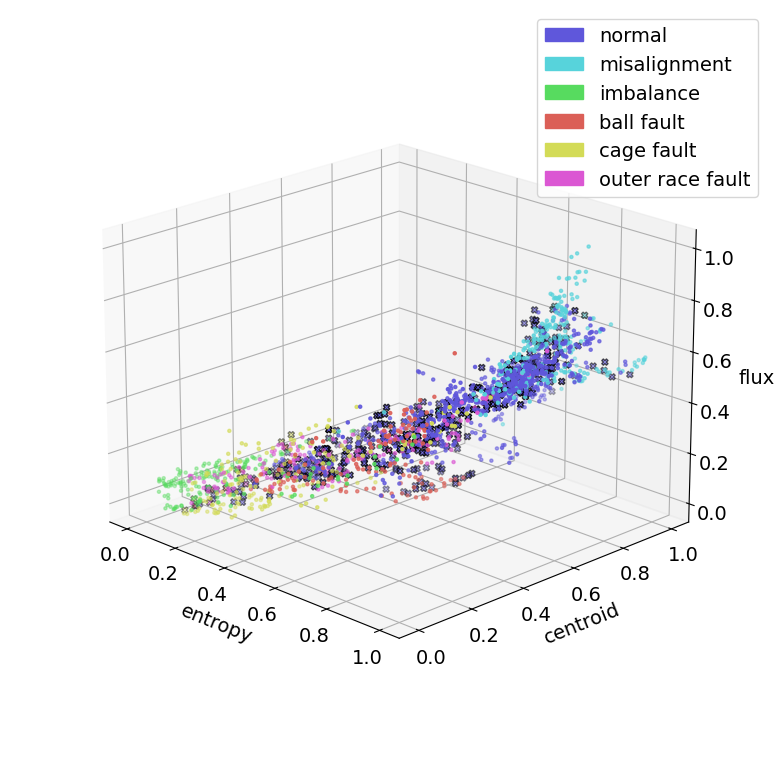
\includegraphics[width=\textwidth]{assets/results/labels/FD-severity.png}
        \caption{Frequency-domain features (severity) [91.24\%]}
    \end{subfigure} 
    \caption{Three features chosen by rank product, ranges of attributes, and prediction accuracy in brackets}
\end{figure}

The features chosen by rank product are visualized as a three-dimensional scatter plot. The colors of data points represent correct labels with ex marks for misses. The scales on graph axes are inverse transformed of the min-max scaler. The visualization of predicted groups suggests another transform should be applied to even out the distances and handle the outliers.


\subsection{Incremental learning}
Online learning imitates hardened conditions for machinery diagnostics that appear in deployment. Delayed provision or omission of actual labels undoubtedly degrades the reliability of the classification. The question is how quickly the accuracy approaches the optimal one from the nearest neighbors trained in batch and what is the effect on the k-NN model from routine difficulties associated with the continous labeling process.

\begin{figure}[h]
    \centering
    \begin{subfigure}[b]{0.32\textwidth}
        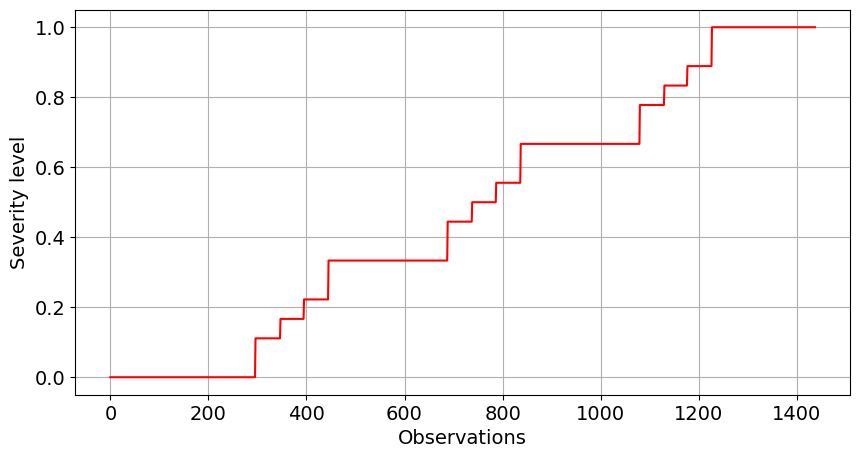
\includegraphics[width=\textwidth]{assets/results/incremental-learning/severity-levels.png}
        \caption{Relative severity levels}
        \label{fig:design:online-count-severity-level}
    \end{subfigure}
    \hfill
    \begin{subfigure}[b]{0.32\textwidth}
        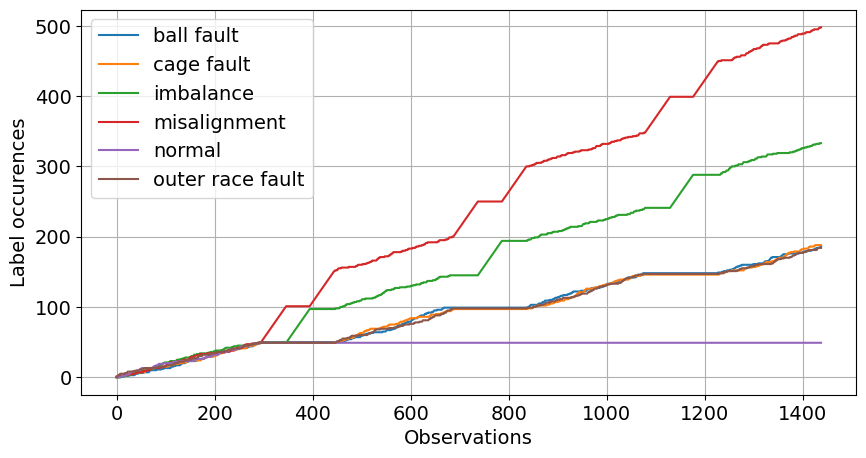
\includegraphics[width=\textwidth]{assets/results/incremental-learning/order-natural.png}
        \caption{Original labels}
        \label{fig:design:online-event-order}
    \end{subfigure}
    \hfill
    \begin{subfigure}[b]{0.32\textwidth}
        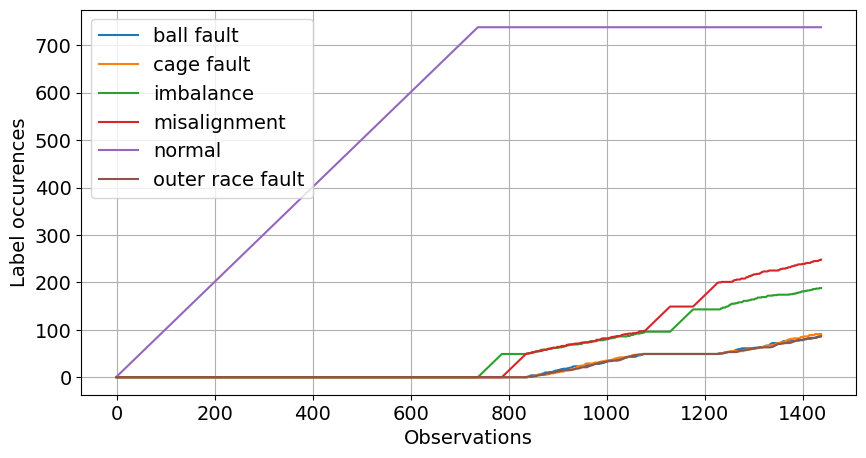
\includegraphics[width=\textwidth]{assets/results/incremental-learning/order-severity.png}
        \caption{High severity labels}
         \label{fig:design:online-event-order-severity}
    \end{subfigure}
    \caption{Ordering of faults in dataset according to relative severity levels}
\end{figure}

The k-NN models in incremental learning experiments learn on the same base training dataset as in batch learning for bearing A with complete sets of extracted features. In this manner, we can compare the training accuracies in the last sample for both models. Online learning metrics are evaluated by progressive valuation on a dataset that is left unbalanced.

The \textbf{stream of events} is ordered by rising severity levels (Fig.~\ref{fig:design:online-count-severity-level}), which ensures steady increments in label counts throughout the simulation (Fig.~\ref{fig:design:online-event-order}). The same sorting approach is applied to the dataset where low-severity faults are annotated as baseline observations. During most of its lifespan, the machine simulator looks to be in a fine operating state. Near the end of the simulation, faults start to develop (Fig.~\ref{fig:design:online-event-order-severity}).  

These artificially streamlined event sequences are a bit unrealistic because all types of faults never begin to appear simultaneously with equal strengths. It is meant to approximate the gradual overall degradation of the machine.


%
%Major breaking points in the stream are after 1171 observations out of 5751, where all 203 normal conditions are consumed in the training process. Counters of other faults show that model predictions are skewed towards more represented classes of imbalance and misalignement. The uneven evolution of category counts in a stream impacts the development of accuracy in the remaining experiments. The hold-out validation accuracies of comparable batch models are 97.36\% \emph{(temporal features)} and 98.36\% \emph{(spectral features)}.
%	
%During gradual learning, the correct label is supplied after a fixed period passes after its prediction. This \textbf{sliding window} simulation examines accuracy every 100 iterations. Wait times before revealing the actual class associated with the sample are 1, 50, 100, or 250 steps (Fig.~\ref{fig:design:online-fault-delay-sliding}). 
%
%
%Accuracies after sequentially seeing all samples 96.78\% in temporal domain and 89.11\% in spectral domain when labels are shown instantly. Scatter plots in Figure~\ref{fig:design:scatter-plot-online} visualize mistakes in predictions projected onto two principal components. Labeling delay of 250 observations causes accuracy to drop to 83.94\% \emph{(temporal)} and 78.81\% \emph{(spectral)}.
%
%	
%In the final sample, the accuracies are 89.11\% \emph{(temporal)} and 90.38\% \emph{(spectral)} with immediate feedback, and 83.08\% \emph{(temporal)} and 85.01\% \emph{(spectral)} with window length of 250 samples (Fig.~\ref{fig:design:online-fault-delay-tumbling}). 
%
%A \textbf{tumbling window} is more accurate according to progressive valuation because the labeling delay decreases towards the window's end. Initial 0\% accuracy is caused by a warming-up period in data collection during the span of the first few windows. The true labels are unknown. After just a handful of windows in the beginning, accuracy jumps above 60\% and stabilizes after 1000 observations.
%
% 
%Labeling just every \nth{5} sample (25\% of the total dataset) with a sliding window delay of 10 samples reduces accuracy for the model out of temporal features by 8.41\% to 80.39\%, and by 7.33\% for spectral features to accuracy of 82.01\% (Fig.~\ref{fig:design:online-label-skip}). Even if only 1\% of the dataset is annotated (every \nth{100} sample), the model out of spectral features retained an accuracy of 65.17\% that is 4.41\% better than for temporal features.  More missing labels require recording more observations before the equivalent accuracy is reached.






% Tumbling windows
\begin{figure}[h]
    \centering
    \begin{subfigure}[b]{0.48\textwidth}
        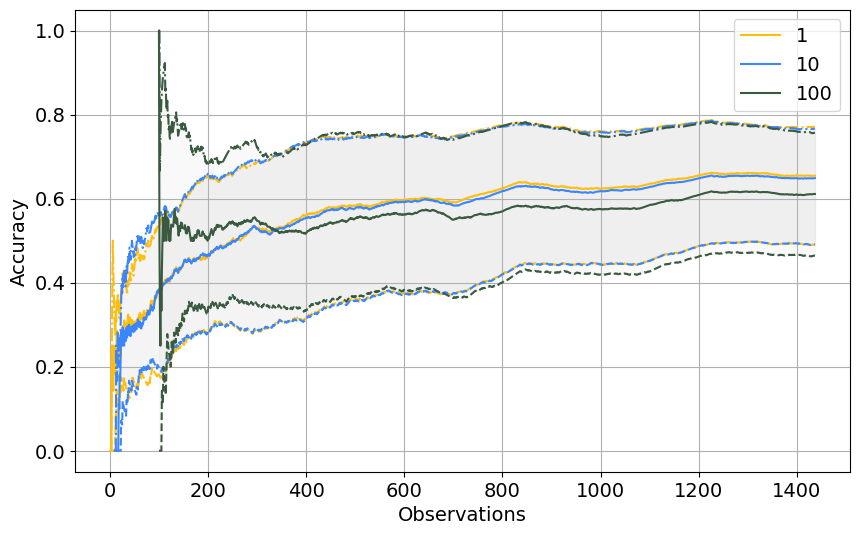
\includegraphics[width=\textwidth]{assets/results/incremental-learning/tumbling-TD.png}
        \caption{Time-domain features}
    \end{subfigure}
    \hfill
    \begin{subfigure}[b]{0.48\textwidth}
        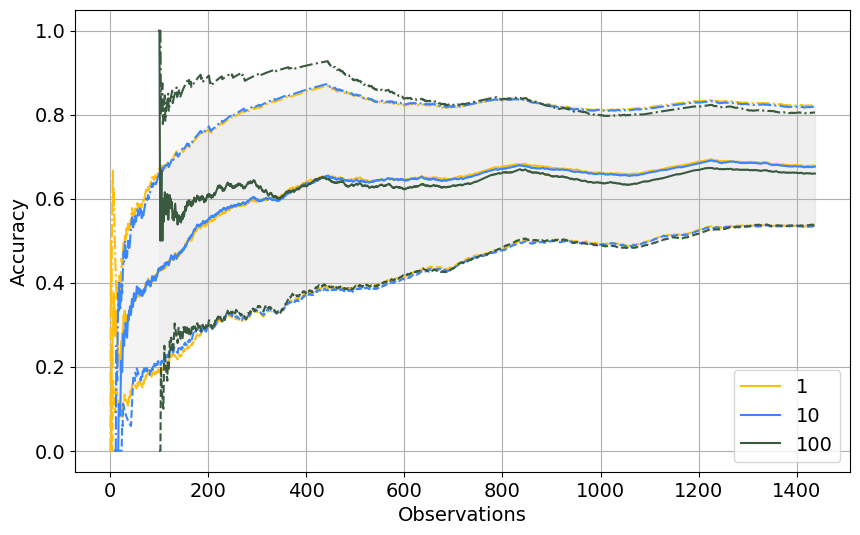
\includegraphics[width=\textwidth]{assets/results/incremental-learning/tumbling-FD.png}
        \caption{Frequency-domain features}
    \end{subfigure}
    \hfill
    \begin{subfigure}[b]{0.48\textwidth}
        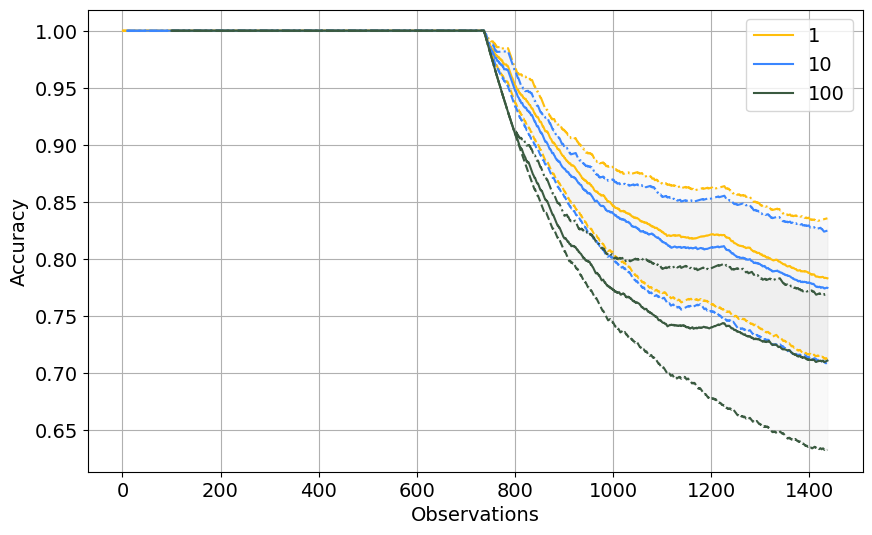
\includegraphics[width=\textwidth]{assets/results/incremental-learning/tumbling-TD-severity.png}
        \caption{Time-domain features (severity)}
    \end{subfigure}
    \hfill
    \begin{subfigure}[b]{0.48\textwidth}
        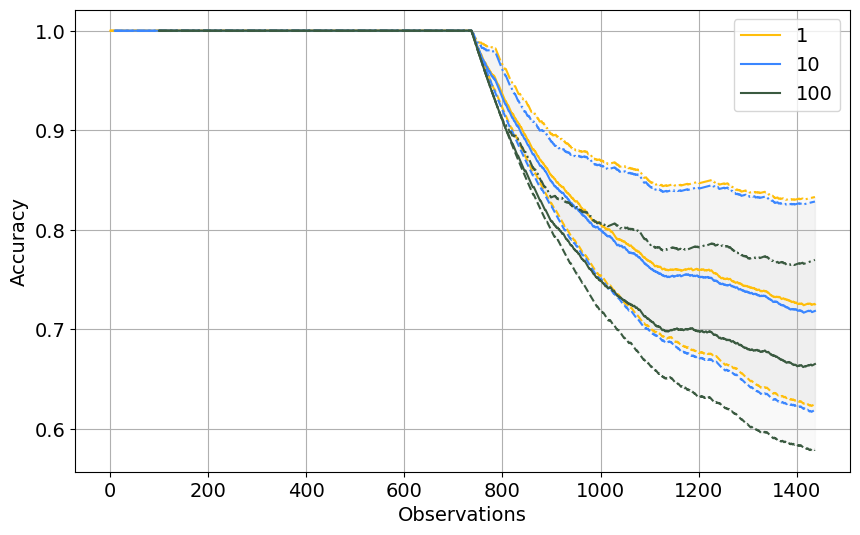
\includegraphics[width=\textwidth]{assets/results/incremental-learning/tumbling-FD-severity.png}
        \caption{Frequency-domain features (severity)}
    \end{subfigure} 
    \caption{Tumbling window in incremental learning}
\end{figure}


% % Label skips and parts of dataset
\begin{figure}[h]
    \centering
    \begin{subfigure}[b]{0.48\textwidth}
        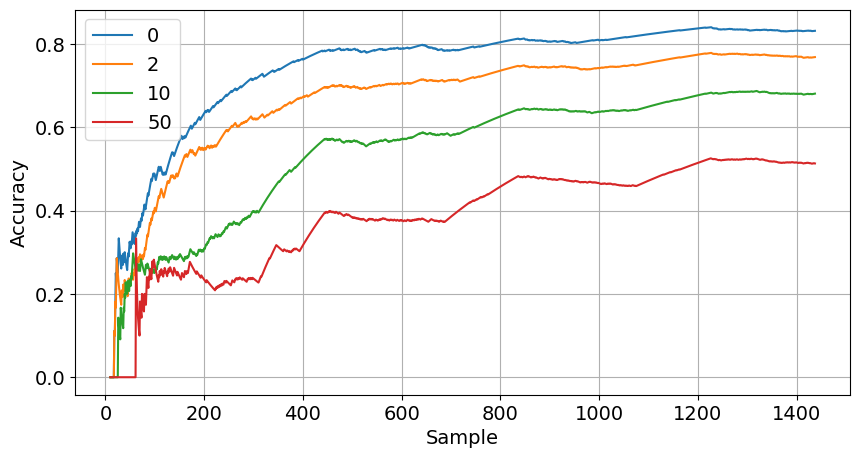
\includegraphics[width=\textwidth]{assets/results/incremental-learning/all-features-TD-skip.png}
        \caption{Time-domain features}
    \end{subfigure}
    \hfill
    \begin{subfigure}[b]{0.48\textwidth}
        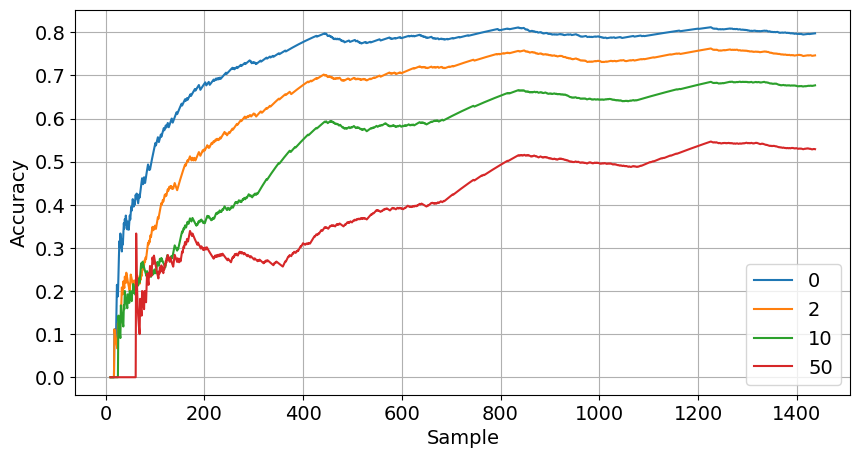
\includegraphics[width=\textwidth]{assets/results/incremental-learning/all-features-FD-skip.png}
        \caption{Frequency-domain features}
    \end{subfigure}
    \hfill
    \begin{subfigure}[b]{0.48\textwidth}
        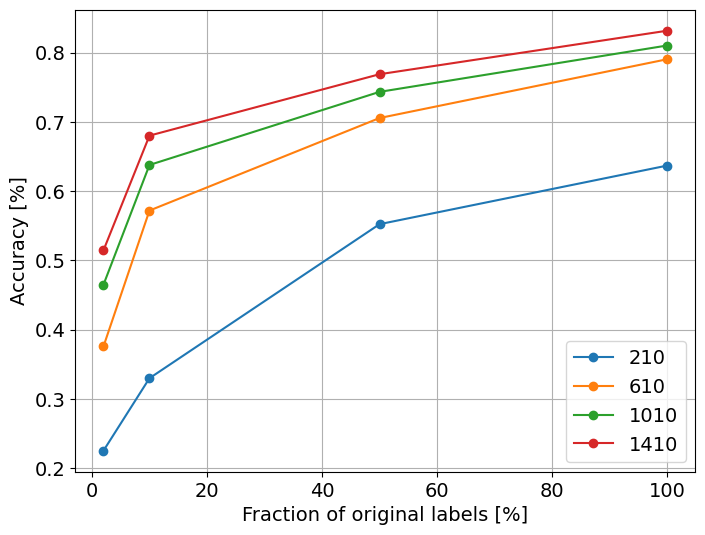
\includegraphics[width=\textwidth]{assets/results/incremental-learning/skip-labels-TD.png}
        \caption{Time-domain features}
    \end{subfigure}
    \hfill
    \begin{subfigure}[b]{0.48\textwidth}
        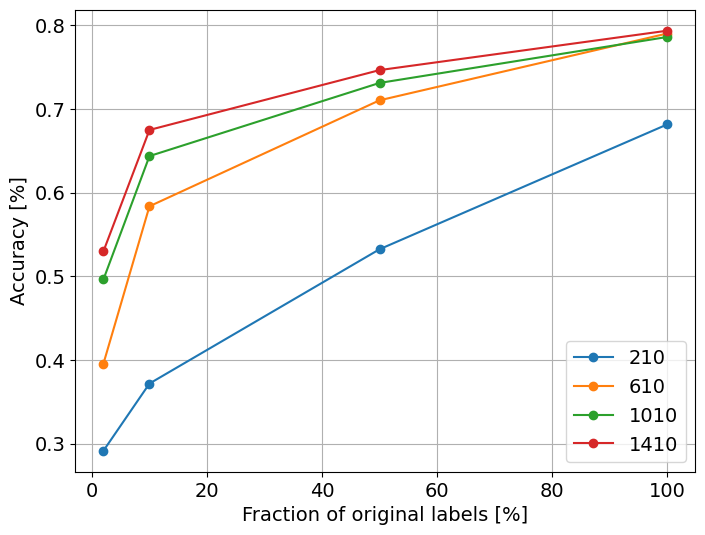
\includegraphics[width=\textwidth]{assets/results/incremental-learning/skip-labels-FD.png}
        \caption{Frequency-domain features}
    \end{subfigure} 
    \caption{Skip labels in incremental learning}
\end{figure}


\begin{figure}[h]
    \centering
    \begin{subfigure}[b]{0.48\textwidth}
        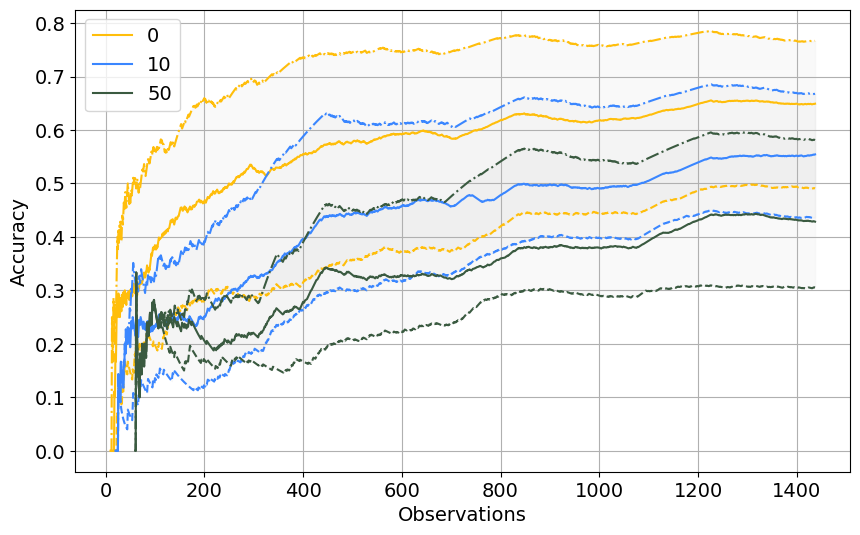
\includegraphics[width=\textwidth]{assets/results/incremental-learning/skip-label-TD.png}
        \caption{Time-domain features}
    \end{subfigure}
    \hfill
    \begin{subfigure}[b]{0.48\textwidth}
        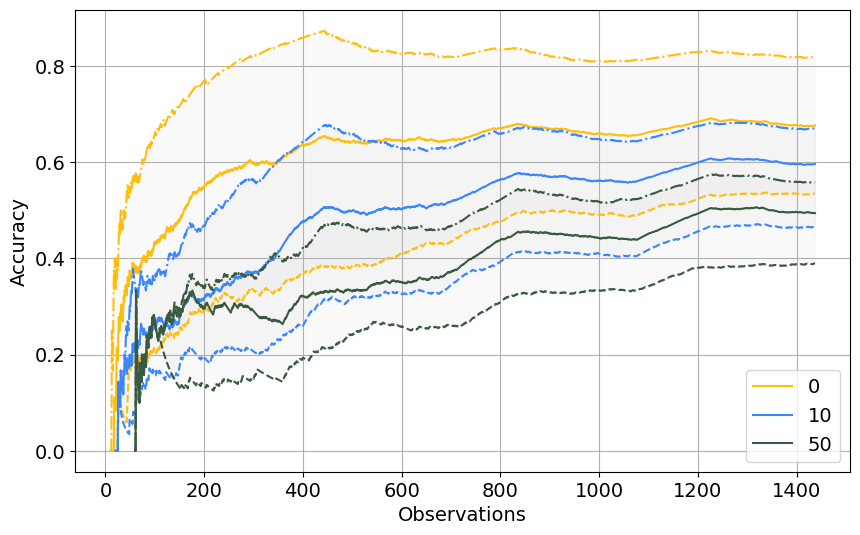
\includegraphics[width=\textwidth]{assets/results/incremental-learning/skip-label-FD.png}
        \caption{Frequency-domain features}
    \end{subfigure}
    \hfill
    \begin{subfigure}[b]{0.48\textwidth}
        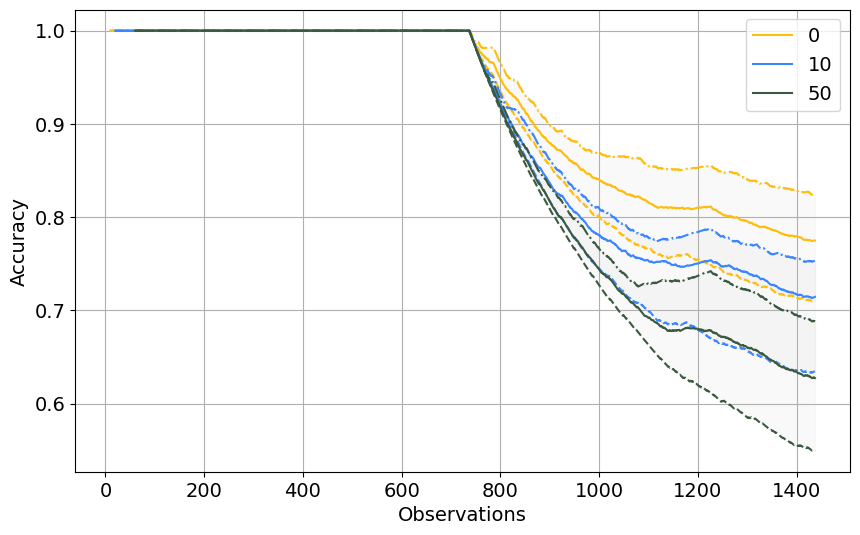
\includegraphics[width=\textwidth]{assets/results/incremental-learning/skip-label-TD-severity.png}
        \caption{Time-domain features (severity)}
    \end{subfigure}
    \hfill
    \begin{subfigure}[b]{0.48\textwidth}
        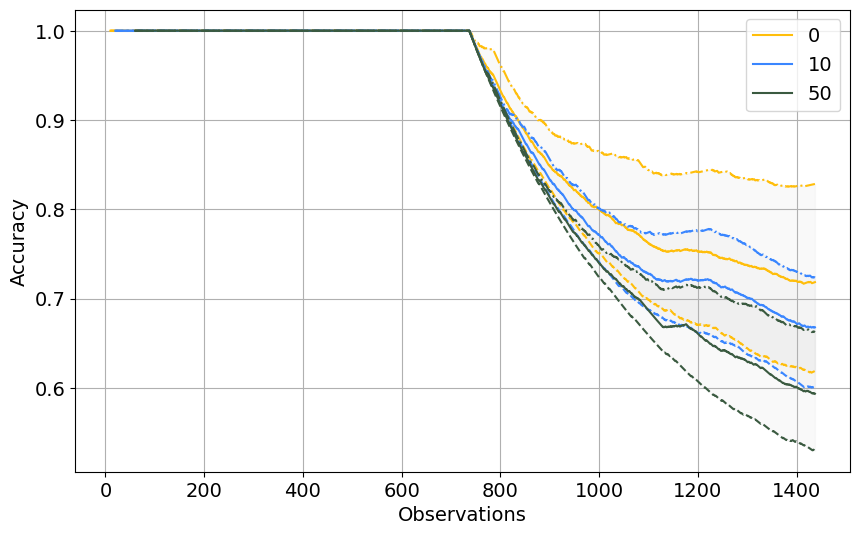
\includegraphics[width=\textwidth]{assets/results/incremental-learning/skip-label-FD-severity.png}
        \caption{Frequency-domain features (severity)}
    \end{subfigure} 
    \caption{Skip labels in incremental learning with different sizes}
\end{figure}



\section{Industrial dataset analysis}

\subsection{Data logger validation}

\begin{figure}[h]
    \centering
    \begin{subfigure}[b]{0.49\textwidth}
        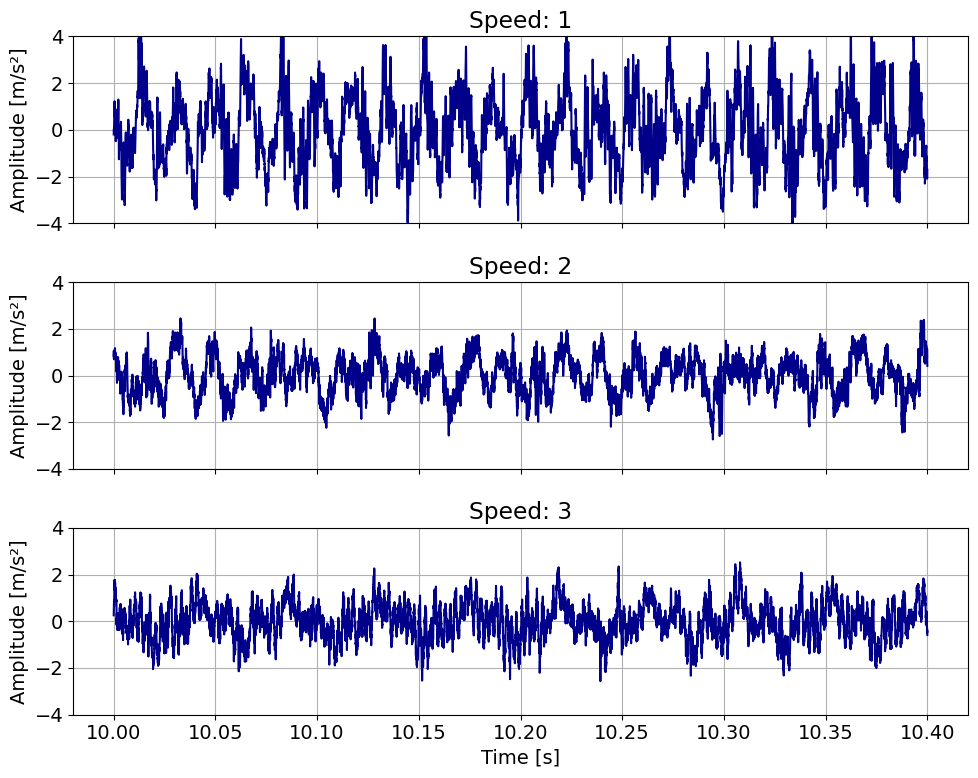
\includegraphics[width=\textwidth]{assets/results/standing-fan/waveform.png}
        \caption{Time waveform}
    \end{subfigure}
    \hfill
    \begin{subfigure}[b]{0.49\textwidth}
        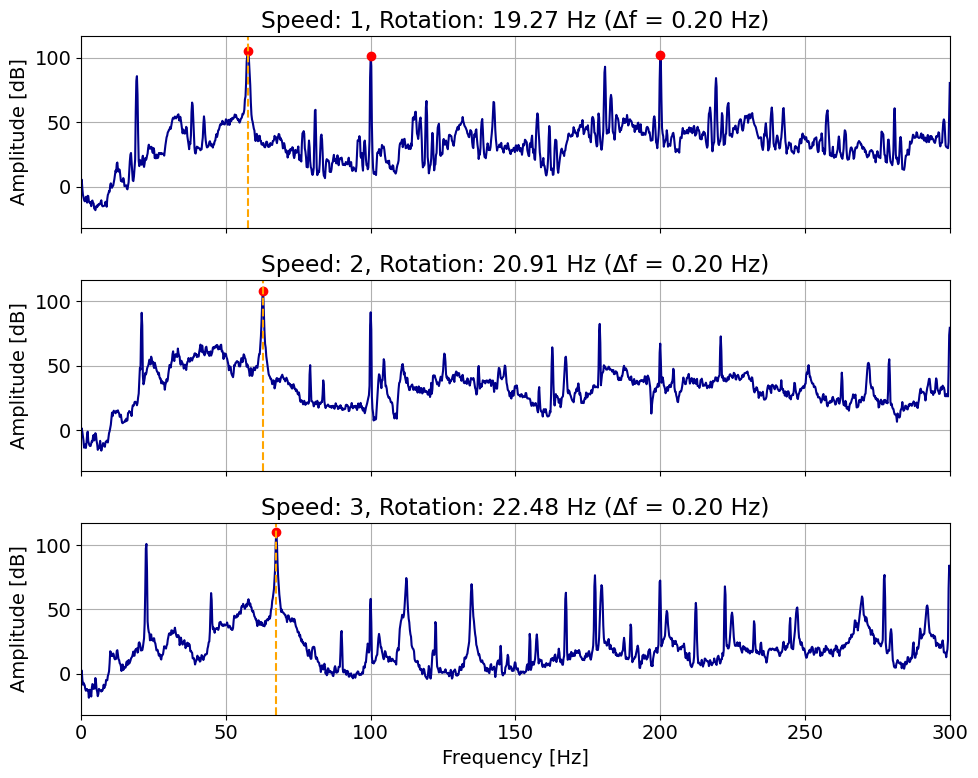
\includegraphics[width=\textwidth]{assets/results/standing-fan/standing-fan-accel.png}
        \caption{Estimation of rotation speed}
    \end{subfigure}
    \caption{Vibrations from the back of a standing fan in radial direction}
\end{figure}


\subsection{Feature ranges}
% Amplitude histograms - 20m/s^2, 40m/s^2, 150m/s^
% Histograms of machinery measurements


% Box plots of features
\begin{figure}[h]
    \centering
    \begin{subfigure}[b]{\textwidth}
        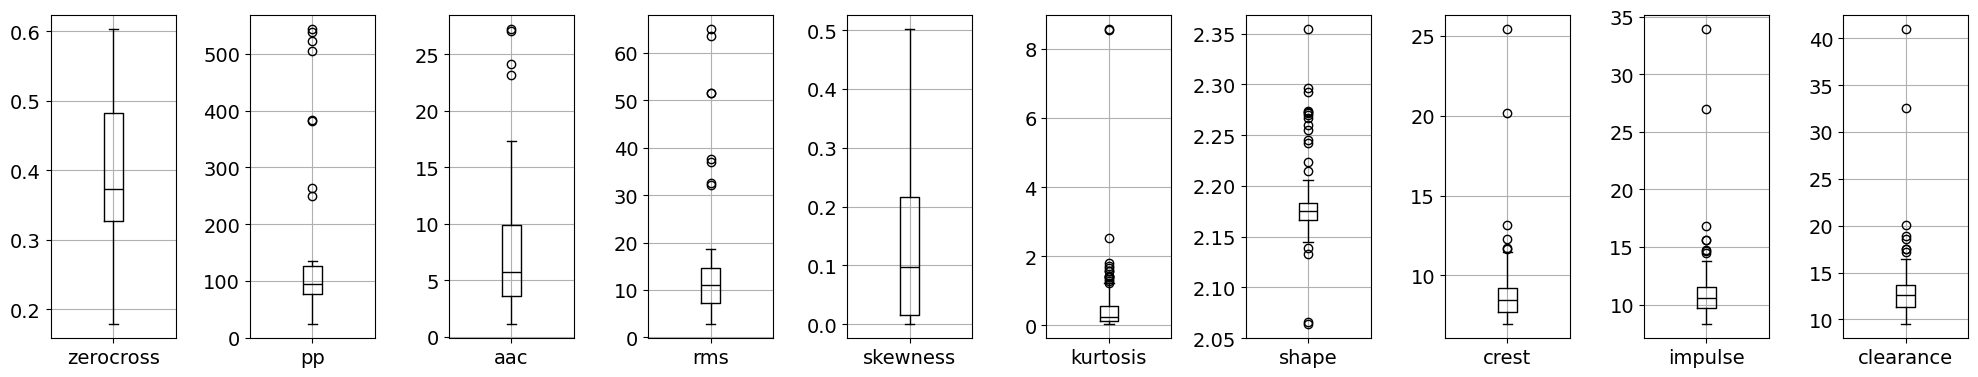
\includegraphics[width=\textwidth]{assets/results/feature-values/pumps-TD-dim-3.png}
        \caption{Time-domain features}
    \end{subfigure}
    \hfill
    \begin{subfigure}[b]{\textwidth}
        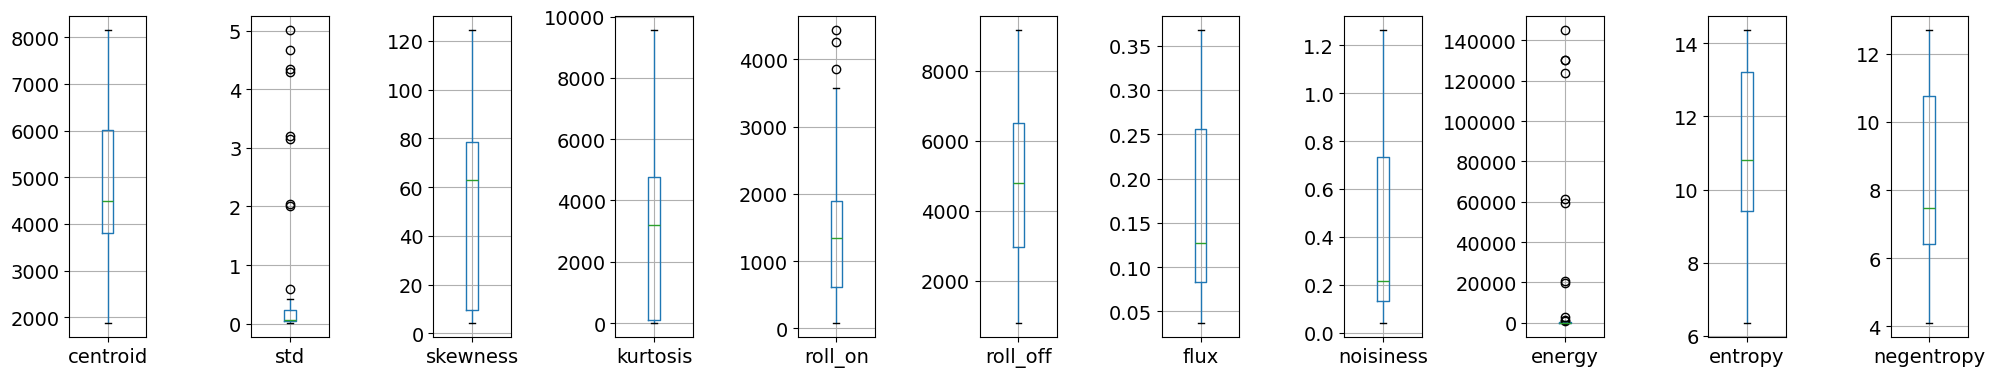
\includegraphics[width=\textwidth]{assets/results/feature-values/pumps-FD-dim-3.png}
        \caption{Frequency-domain features}
    \end{subfigure}
    \caption{Feature range in pumps}
\end{figure}

\subsection{Time-frequency waveforms}
\begin{figure}[h]
    \centering
    \begin{subfigure}[b]{0.32\textwidth}
        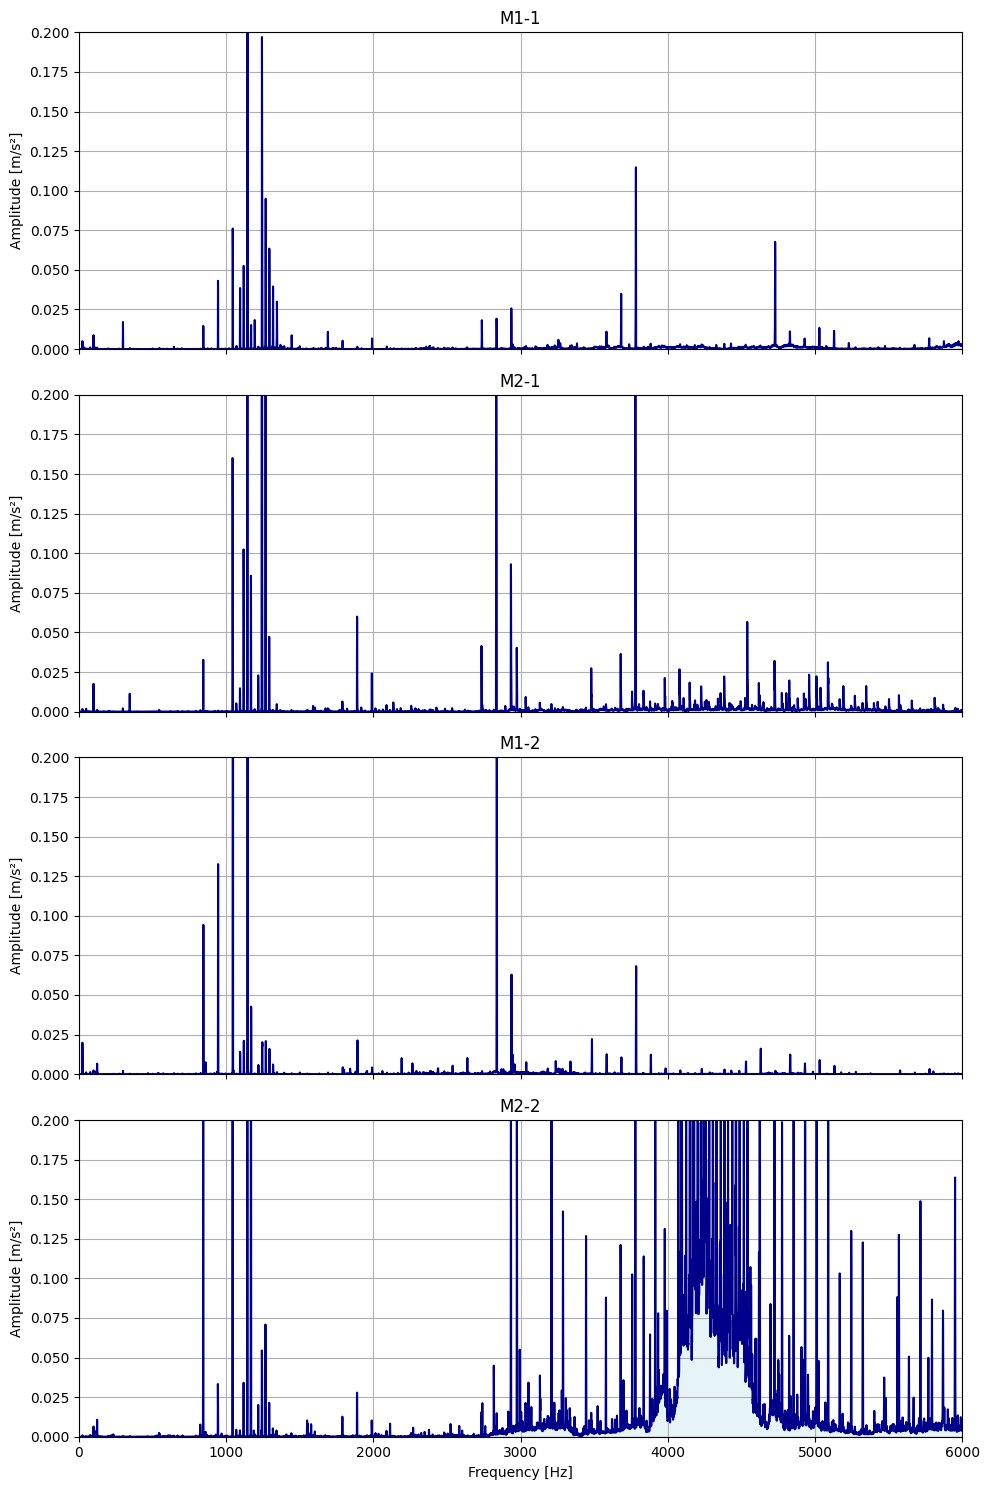
\includegraphics[width=\textwidth]{assets/results/eda/frequency-spectrum-motors.png}
        \caption{Motors}
    \end{subfigure}
    \hfill
    \begin{subfigure}[b]{0.32\textwidth}
        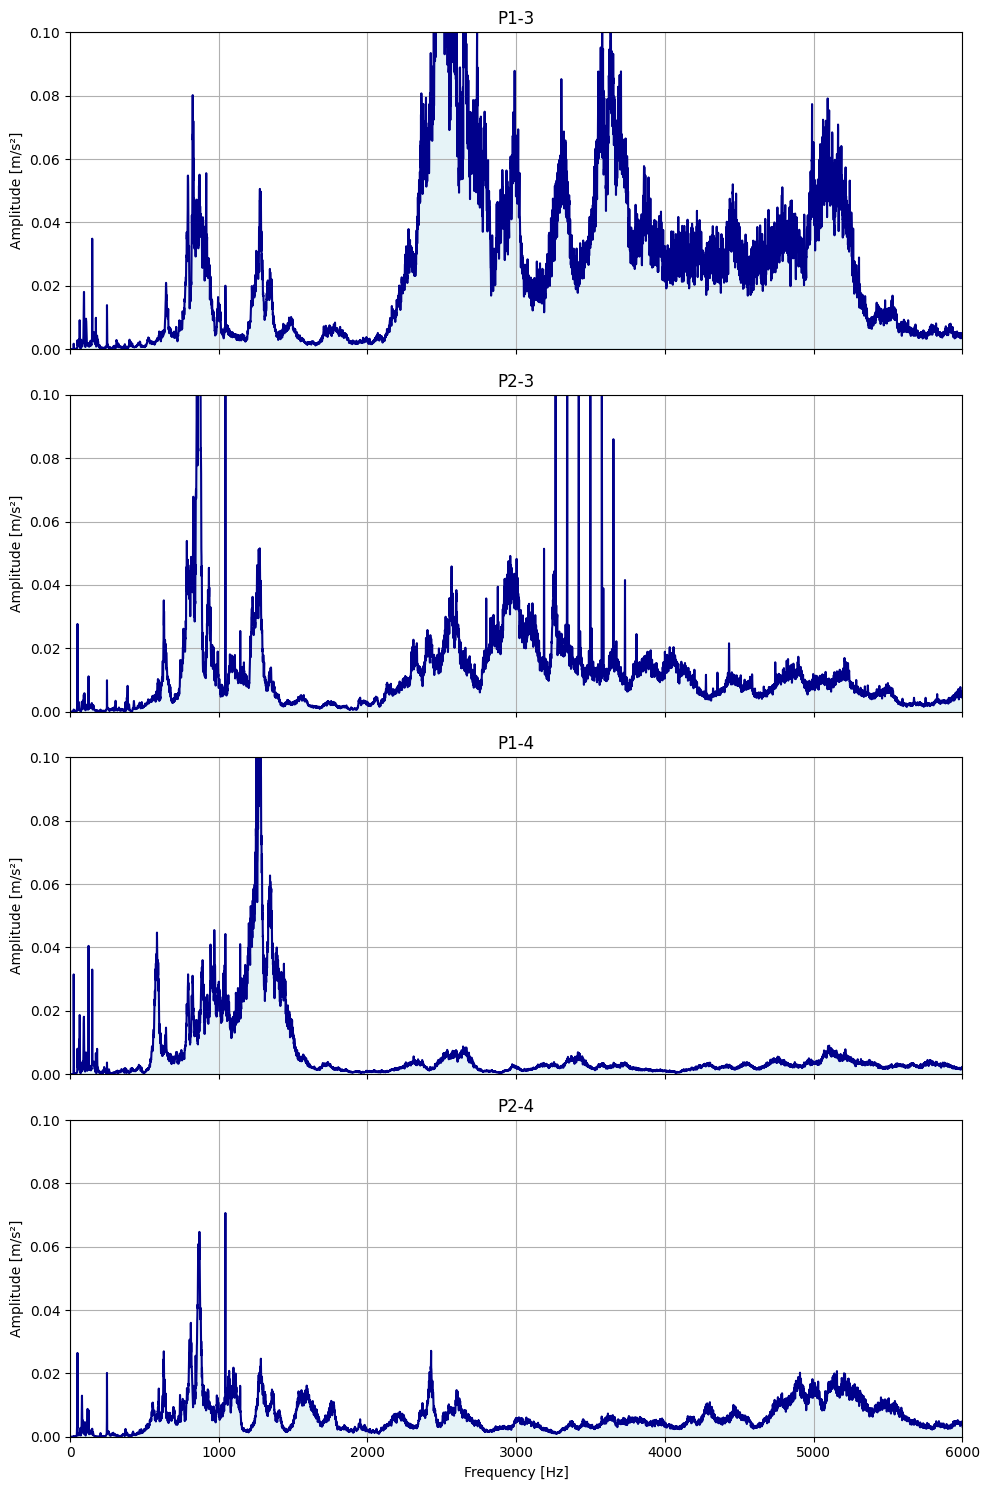
\includegraphics[width=\textwidth]{assets/results/eda/frequency-spectrum-pumps.png}
        \caption{Pumps}
    \end{subfigure}
    \hfill
    \begin{subfigure}[b]{0.32\textwidth}
        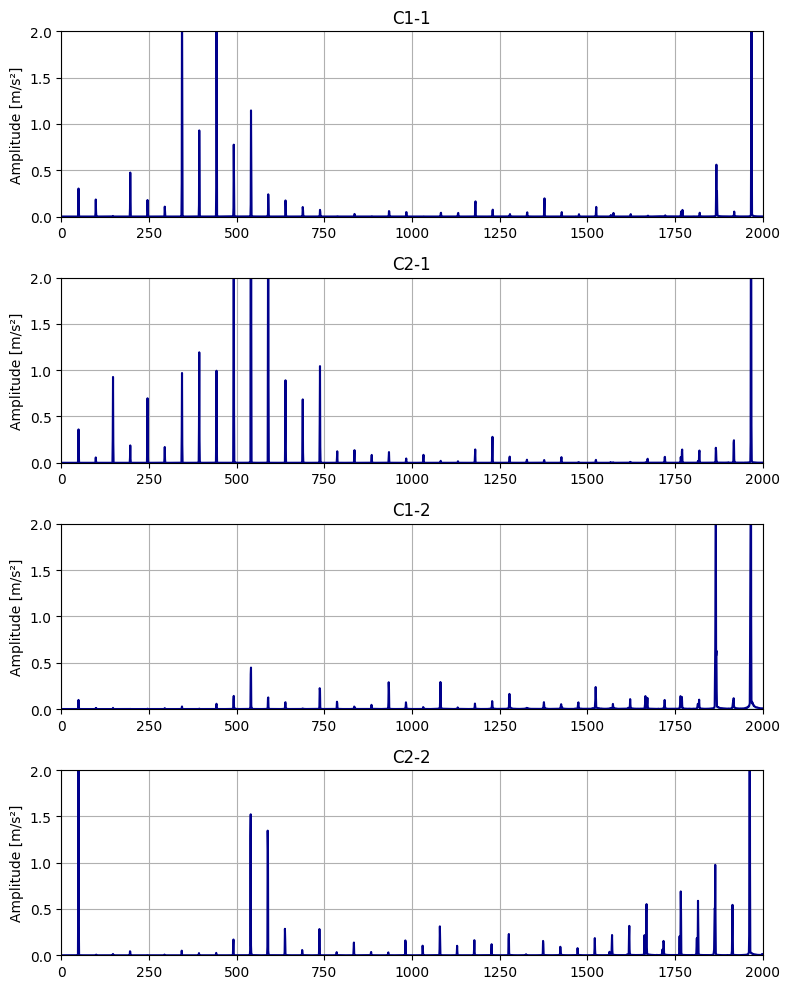
\includegraphics[width=\textwidth]{assets/results/eda/frequency-spectrum-compressors.png}
        \caption{Compressor}
    \end{subfigure} 
    \caption{Frequency domain}
\end{figure}


% Time-frequency spectrum

% Low frequencies (under 1KHz)

\begin{figure}[h]
    \centering
    \begin{subfigure}[b]{0.48\textwidth}
        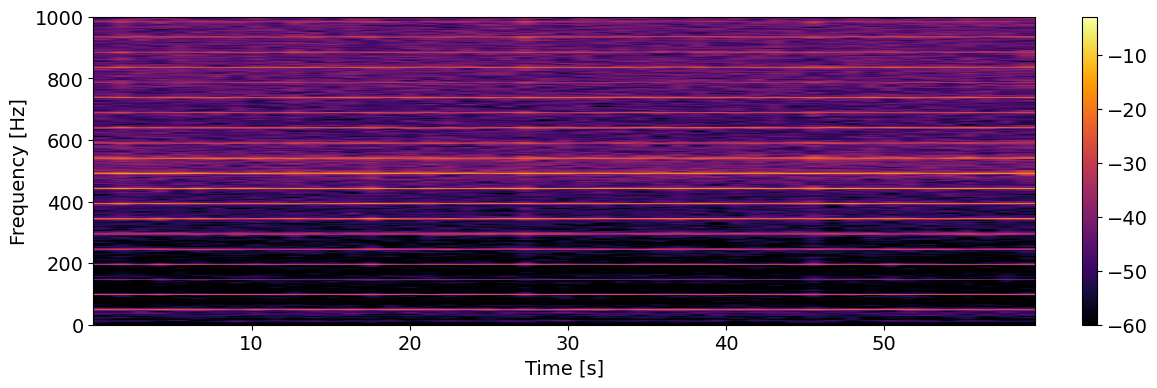
\includegraphics[width=\textwidth]{assets/results/time-frequency-spectrum/K3-z-STFT-1kHz.png}
        \caption{K3}
    \end{subfigure}
    \hfill
    \begin{subfigure}[b]{0.48\textwidth}
        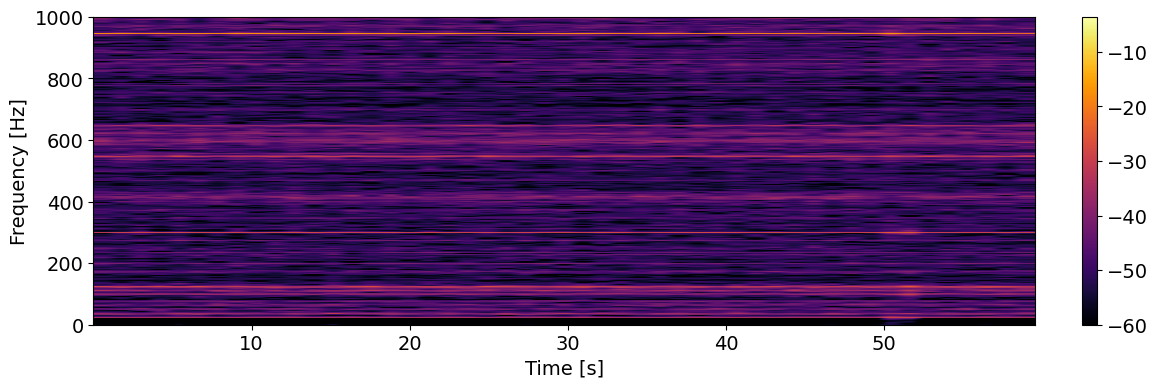
\includegraphics[width=\textwidth]{assets/results/time-frequency-spectrum/M1-2-z-STFT-1kHz.png}
        \caption{M1-2}
    \end{subfigure}
    \hfill
    \begin{subfigure}[b]{0.48\textwidth}
        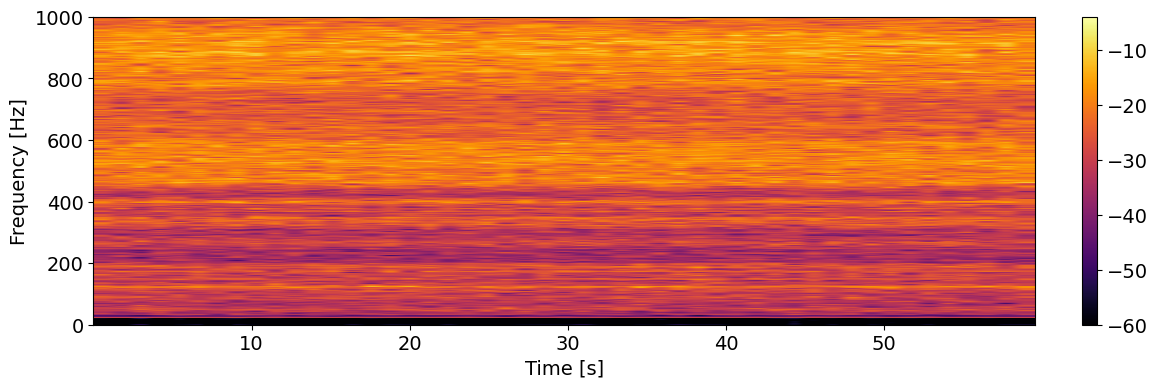
\includegraphics[width=\textwidth]{assets/results/time-frequency-spectrum/P1-3-z-STFT-1kHz.png}
        \caption{P1-3}
    \end{subfigure}
	\hfill
	\begin{subfigure}[b]{0.48\textwidth}
        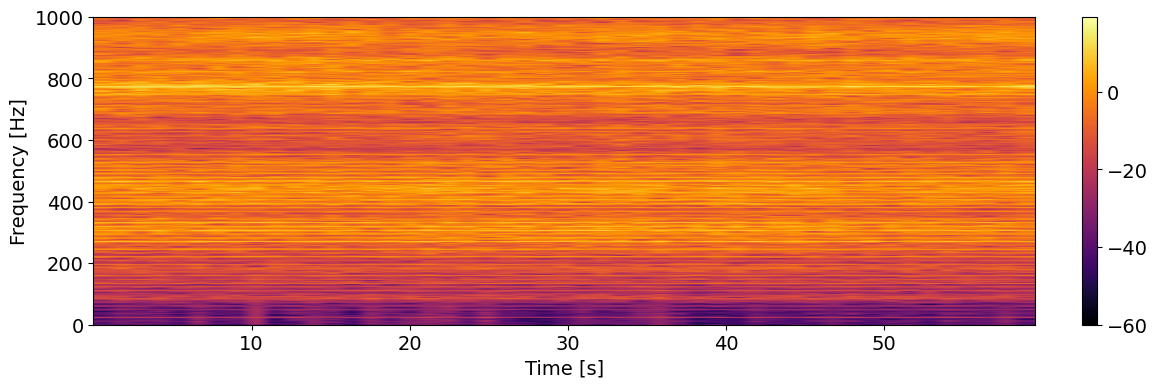
\includegraphics[width=\textwidth]{assets/results/time-frequency-spectrum/P3-3-z-STFT-1kHz.png}
        \caption{P3-3}
    \end{subfigure}
    \caption{Time frequency spectrum}
\end{figure}


\begin{figure}[h]
    \centering
    \begin{subfigure}[b]{0.48\textwidth}
        \includegraphics[width=\textwidth]{assets/results/time-frequency-spectrum/P1-slow-down.png}
        \caption{Pump P1 turns off}
    \end{subfigure}
    \hfill
    \begin{subfigure}[b]{0.48\textwidth}
        \includegraphics[width=\textwidth]{assets/results/time-frequency-spectrum/P2-speed-up.png}
        \caption{Pump P2 turn on}
    \end{subfigure}
\end{figure}

\subsection{Bearing defect frequencies}
% Domain expert analysis
% Bearing frequencies table
\begin{table}[h]
\centering
\begin{tabular}{|l|r|r|r|}
\hline
\textbf{Placement}     & \multicolumn{1}{l|}{\textbf{Motor \#1}} & \multicolumn{1}{l|}{\textbf{Motor \#2}} & \multicolumn{1}{l|}{\textbf{Pump \#3 \& \#4}} \\ \hline
\textbf{Bearing}       & \multicolumn{1}{l|}{6319-C3}            & \multicolumn{1}{l|}{6324-C3}            & \multicolumn{1}{l|}{6317-2Z}                  \\ \hline
\textbf{$n$}           & 8                                       & 8                                       & 8                                             \\ \hline
\textbf{$f_s$}         & 1493                                    & 1493                                    & 1493                                          \\ \hline
\textbf{$d$ {[}mm{]}}  & 33.12                                   & 41.28                                   & 30.00                                         \\ \hline
\textbf{$D$ {[}mm{]}}  & 147.5                                   & 190.0                                   & 132.5                                         \\ \hline
\textbf{$\beta$}       & 0                                       & 0                                       & 0                                             \\ \hline
\textbf{RPM {[}Hz{]}}  & 24.88                                   & 24.88                                   & 24.88                                         \\ \hline
\textbf{BPFO {[}Hz{]}} & 77.18                                   & 77.91                                   & 77.00                                         \\ \hline
\textbf{BPFI {[}Hz{]}} & 121.88                                  & 121.16                                  & 122.07                                        \\ \hline
\textbf{BSF {[}Hz{]}}  & 58.20                                   & 59.97                                   & 57.77                                         \\ \hline
\textbf{FTF {[}Hz{]}}  & 9.65                                    & 9.74                                    & 9.63                                          \\ \hline
\end{tabular}
\end{table}

% Bearing defect frequencies
\begin{figure}[h]
    \centering
    \begin{subfigure}[b]{0.24\textwidth}
        \includegraphics[width=\textwidth]{assets/results/defects/motors.png}
        \caption{Motors}
    \end{subfigure}
    \hfill
    \begin{subfigure}[b]{0.24\textwidth}
        \includegraphics[width=\textwidth]{assets/results/defects/motors-dB.png}
        \caption{Pumps}
    \end{subfigure}
    \begin{subfigure}[b]{0.24\textwidth}
        \includegraphics[width=\textwidth]{assets/results/defects/pumps.png}
        \caption{Motors}
    \end{subfigure}
    \hfill
    \begin{subfigure}[b]{0.24\textwidth}
        \includegraphics[width=\textwidth]{assets/results/defects/pumps-dB.png}
        \caption{Pumps dB}
    \end{subfigure}
\end{figure}


\subsection{Pump long-term monitoring}

% Total vibration levels - challange - long-live span (5 years)
\begin{figure}[h]
    \centering
    \begin{subfigure}[b]{0.49\textwidth}
        \includegraphics[width=\textwidth]{assets/results/ksb-cloud/p1.png}
        \caption{Pump P1}
    \end{subfigure}
    \hfill
    \begin{subfigure}[b]{0.49\textwidth}
        \includegraphics[width=\textwidth]{assets/results/ksb-cloud/p2.png}
        \caption{Pump P2}
    \end{subfigure}
    \caption{Vibration levels}
\end{figure}

% Reverse engineer of spectra (low resolution)
\begin{figure}[h]
    \centering
    \includegraphics[width=0.8\textwidth]{assets/results/ksb-cloud/spectrum.png}
    \caption{Frequency spectrum}
\end{figure}


